%\PassOptionsToPackage{table}{xcolor}
\documentclass[
	a4paper,
	12pt,
	oneside,
	%twoside,
	%openright,
	final
	%draft,				% Entwurf: Druckt keine Bilder
]{scrreprt}

\usepackage[T1]{fontenc}
\usepackage[utf8]{inputenc}
\usepackage[ngerman]{babel}
\usepackage{booktabs}
\usepackage{textcomp}
\usepackage{mathptmx}
\usepackage{bibentry}
\usepackage{helvet}
\usepackage[hyperfootnotes=false]{hyperref}	
\usepackage{makeidx}
\usepackage{listings}
\usepackage{color}
\usepackage[usenames,dvipsnames]{xcolor}
\usepackage{natbib}
\usepackage{fancyhdr}
\usepackage[smaller]{acronym}
\usepackage{tabularx}
\usepackage{ntheorem}
\usepackage{array}
\usepackage{caption}
\usepackage{relsize}
\usepackage{graphicx}
\usepackage{Includes/stmaryrd/stmaryrd}
\usepackage{subfig}
\usepackage{pst-all, pst-circ, pst-fill}
\usepackage{Includes/tikz/tex/latex/pgf/frontendlayer/tikz}
\include{Includes/tikz/tex/generic/pgf/frontendlayer/tikz/libraries/pgflibrarytikzshadows.code.tex}
\usetikzlibrary{arrows,shadows,patterns} % for pgf-umlsd
\usepackage{Includes/pgf-umlsd}
\usepackage{uml}
\usepackage{attrib}
\usepackage{longtable}	

\setcounter{tocdepth}{2}
\setcounter{secnumdepth}{4}

% Einrückung der ersten Zeile eines Absatzes
%\parindent3mm
\usepackage{setspace}
%\setstretch{1}
\linespread{1.15}

\colorlet{chapter}{black!75}
\addtokomafont{chapter}{\color{chapter}}
%
\makeatletter% siehe De-TeX-FAQ
\renewcommand*{\chapterformat}{%
  \begingroup% damit \unitlength-Änderung lokal bleibt
    \setlength{\unitlength}{1mm}%
   % \begin{picture}(20,10)(0,5)
	\begin{picture}(20,40)(0,5)%     
      \setlength{\fboxsep}{0pt}
%      \put(0,0){\framebox(20,40){}}%
%      \put(0,20){\makebox(20,20){\rule{20\unitlength}{20\unitlength}}}%
      \put(20,15){\line(1,0){\dimexpr
          \textwidth-20\unitlength\relax\@gobble}}%
      \put(0,0){\makebox(20,20)[r]{%
          \fontsize{28\unitlength}{28\unitlength}\selectfont\thechapter
          \kern-.05em% Ziffer in der Zeichenzelle nach rechts schieben
        }}%
      \put(20,15){\makebox(\dimexpr
          \textwidth-20\unitlength\relax\@gobble,\ht\strutbox\@gobble)[l]{%
            \ \normalsize\color{black}\chapapp~\thechapter\autodot
          }}%
    \end{picture} % <-- Leerzeichen ist hier beabsichtigt!
  \endgroup
}
\makeatother% siehe \makeatletter



% Title page information
\title{Identifikation von fehlerbehafteten Daten zur energiebewu\ss ten Programmierung}
\author{Ren\'{e} Frank}
%\supervisor{Dipl.-Inf. Pablo Graubner}
%\reader{Prof. Dr. Bernd Freisleben}

% Setzen der Meta-Daten
\hypersetup{
	pdftitle={Identifikation von fehlerbehafteten Daten zur energiebewu\ss ten Programmierung},
	pdfauthor={Ren\'{e} Frank},
	pdfkeywords={Bachelorarbeit, },
	pdfsubject={Bachelorarbeit}
}

% Konfiguration der Listings im Dokument
\renewcommand{\ttdefault}{pcr}\par 		

\lstdefinestyle{stJava}{basicstyle=\footnotesize\ttfamily,
	classoffset=0,	
	numbers=left, 				% show line numbers on the left
	stepnumber=1, 				% show every  line number
	numberstyle=\small, 			% font sitze of line numbers
	numbersep=5pt, 				% separation to the text
	language=Java,				% language of source
	basicstyle=\footnotesize\ttfamily,	% generic style
	backgroundcolor={\color{Sand}},
	stringstyle=\color{blue},		% style of strings
	emphstyle=\color{red},			% sytle of ???
	commentstyle=\color{gray},		% style of comments
	keywordstyle=\bfseries,			% style of keywords
	captionpos=b,
	tabsize=4,				% indentation
	showspaces=false,			% show spaces
	showtabs=false,				% show tabs
	showstringspaces=false,			% show spaces in strings
	breaklines=true,			% breaks long lines
	keywordstyle=\color{LLila},          % keyword style
	morekeywords={enum},
  	%stringstyle=\color{mauve},         % string literal style
  	escapeinside={\%*}{*)},           % if you want to add LaTeX within your code
  	classoffset=1,
	morekeywords={RANDOM, LOSS, ZERO, BITFLIP, BITFLIPB, NONE},keywordstyle=\color{blue}\textit,
	classoffset=0
	%frame=tbl 				% can be: none, single, trbl (or trBL, ...), shadowbox	      		
%    keywordstyle=\color{blue}\bfseries,
}


\lstdefinestyle{stBash}
{	
	language=Bash,
	backgroundcolor=\color{white},
	keywordstyle=\color{BlueViolet}\bfseries,
	commentstyle=\color{Gray},
	stringstyle=\color{Red},
	showstringspaces=false,
	basicstyle=\footnotesize\color{DarkGrey},
	numbers=none,
	captionpos=b,
	frame=tbl,
	tabsize=4,
	breaklines=true
}

\lstnewenvironment{code}
   {
     \lstset{style=stJava,
      xleftmargin=0pt,
      xrightmargin=0pt
    }} {}


% Festlegung Art der Zitierung - Havardmethode: Abkuerzung Autor + Jahr
\bibliographystyle{alpha}
\nobibliography*

% Zeilenabstand
%\usepackage{setspace}
%\doublespacing    % doppelzeilig oder
%\onehalfspacing  % anderthalbzeilig

% Hurenkinder und Schusterjungen werden vermieden
\clubpenalty = 10000
\widowpenalty = 10000
\displaywidowpenalty = 10000

%%%%%%%%%%%%%%%%%%%%%%%%%%%%%%%%%%%%%%%%%%%%%%%%%%%%%%%%%%%%%%%%%%%%%
%%% Definitionen
%%%%%%%%%%%%%%%%%%%%%%%%%%%%%%%%%%%%%%%%%%%%%%%%%%%%%%%%%%%%%%%%%%%%%
\definecolor{Sand}{HTML}{FFFFCC}
\definecolor{LLightBlue}{HTML}{CCCCFF}
\definecolor{LLila}{HTML}{870055}
\definecolor{DarkGrey}{rgb}{0.1,0.1,0.1}

\begin{filecontents}{cpuAnno.dat}
% 0.1 0.8 0.4 13.3 0.7 19.6 1.0 0.3 // x*50, y*2
0 0 5 0.8 20 13.3 35 19.6 50 0.3
\end{filecontents} 
\begin{filecontents}{memoryAnno.dat}
% 0.0 10 0.2 10.5 0.3 11 0.6 12 0.7 13 0.8 13.5 1 15.0  // x*50, y*1
0 10 10 11.5 15 11 30 12 35 13 40 13.5 50 15
\end{filecontents}
\begin{filecontents}{misprediction.dat}
% 0.0 10 0.2 10.5 0.3 11 0.6 12 0.7 13 0.8 13.5 1 15.0  // x*50, y*1
0 10 10 11.5 15 11 30 12 35 13 40 13.5 50 15
\end{filecontents}
%%%%%%%%%%%%%%%%%%%%%%%%%%%%%%%%%%%%%%%%%%%%%%%%%%%%%%%%%%%%%%%%%%%%%
%%% End Definitionen
%%%%%%%%%%%%%%%%%%%%%%%%%%%%%%%%%%%%%%%%%%%%%%%%%%%%%%%%%%%%%%%%%%%%%

%%%%%%%%%%%%%%%%%%%%%%%%%%%%%%%%%%%%%%%%%%%%%%%%%%%%%%%%%%%%%%%%%%%%%
%%% Font Style Java in text
\newcommand{\courier}[1]{{\fontfamily{courier-ttf}\selectfont #1}}
%%%%%%%%%%%%%%%%%%%%%%%%%%%%%%%%%%%%%%%%%%%%%%%%%%%%%%%%%%%%%%%%%%%%%

%%%%%%%%%%%%%%%%%%%%%%%%%%%%%%%%%%%%%%%%%%%%%%%%%%%%%%%%%%%%%%%%%%%%%
%%% Retangle color options

\newcommand{\drawRecA}[1]{{\draw[fill=myblue] #1}}
\newcommand{\drawRecB}[1]{{\draw[fill=bleu] #1}}
\newcommand{\drawRecC}[1]{{\draw[fill=vert] #1}}
\newcommand{\drawRecD}[1]{{\draw[fill=violet] #1}}
\newcommand{\drawRecE}[1]{{\draw[fill=orange] #1}}

\newcommand{\drawlegend}{	
	\node at (2.5,5.2) {Blockgr\"o\ss e in Bytes};
	\path[line width=2pt,-,dashed,draw=myblue] 
			(0.2,4.3) -- (0.7,4.3) node[above,pos=0.5,text=black] {1};
	\path[line width=2pt,-,dashed,draw=bleu] 
	        (1.2,4.3) -- (1.7,4.3) node[above,pos=0.5,text=black] {8};
	\path[line width=2pt,-,dashed,draw=vert] 
	        (2.2,4.3) -- (2.7,4.3) node[above,pos=0.5,text=black] {128};
	\path[line width=2pt,-,dashed,draw=violet] 
			(3.2,4.3) -- (3.7,4.3) node[above,pos=0.5,text=black] {1024};
	\path[line width=2pt,-,dashed,draw=orange] 
			(4.2,4.3) -- (4.7,4.3) node[above,pos=0.5,text=black] {2048};
}


%\newcommand{\drawRecA}[1]{{\draw[pattern=north west lines, pattern color=black] #1}}
%\newcommand{\drawRecB}[1]{{\draw[pattern=vertical lines, pattern color=black] #1}}
%\newcommand{\drawRecC}[1]{{\draw[pattern=horizontal lines, pattern color=black] #1}}
%\newcommand{\drawRecD}[1]{{\draw[pattern=north east lines, pattern color=black] #1}}
%\newcommand{\drawRecE}[1]{{\draw[pattern=crosshatch dots, pattern color=black] #1}}

%\newcommand{\drawlegend}{	
%	\node at (2.5,5.2) {Blockgr\"o\ss e};
%	\draw[pattern=north west lines, pattern color=black] 
%		(0.2,4.3) rectangle (0.7,4.1) node[above,pos=0.5,text=black] {1}	;		        
%	\draw[pattern=vertical lines, pattern color=black] 
%		(1.2,4.3) rectangle (1.7,4.1) node[above,pos=0.5,text=black] {8}	;	
%	\draw[pattern=horizontal lines, pattern color=black] 
%		(2.2,4.3) rectangle (2.7,4.1) node[above,pos=0.5,text=black] {128};				
%	\draw[pattern=north east lines, pattern color=black] 
%		(3.2,4.3) rectangle (3.7,4.1) node[above,pos=0.5,text=black] {1024};		
%	\draw[pattern=crosshatch dots, pattern color=black] 
%		(4.2,4.3) rectangle (4.7,4.1) node[above,pos=0.5,text=black] {2024}	;	
%}

%%%%%%%%%%%%%%%%%%%%%%%%%%%%%%%%%%%%%%%%%%%%%%%%%%%%%%%%%%%%%%%%%%%%%

\setlength{\parindent}{0pt}
\begin{document}


\begin{titlepage}
	
\vspace{0.3cm} \noindent\rule{\textwidth}{0.5mm} \vspace{-0.3cm}	
	
\begin{minipage}{19mm} 
    
\includegraphics{graphics/siegel-philipp.eps} 
\end{minipage}
	\hfill	
\begin{minipage}{65mm}	
	\sffamily
	%\noindent\Large\textbf{\input{graphics/siegel-philipp.eps}}  
	
\begin{flushright}
	\scriptsize FACHBEREICH MATHEMATIK UND INFORMATIK

	\vspace{0.25cm}
	
	\scriptsize Arbeitsgruppe Verteilte Systeme
\end{flushright}

\end{minipage}	
 
	
%	\noindent\footnotesize Philipps-Universit\"at Marburg,\\
%	\footnotesize Fachbereich 12: Mathematik und Informatik \hfill \today
	\vspace{0.3cm} \noindent\rule{\textwidth}{0.1mm}\vspace{1cm}
	\rmfamily\normalsize	



\begin{center}
\Large{\textsf{\textbf{Identifikation von fehlerbehafteten Daten zur energiebewu\ss ten Programmierung}}}
 
\vspace{1em}
 
\large{\textsf{Abschlussarbeit zur Erlangung des akademischen Grades}} \\
\Large{\textsf{Bachelor of Science (B.Sc.)}} \\
\large{\textsf{vorgelegt von}}
 
\vspace{0.5em}
 
\textsf{Ren\'{e} Frank}
 
\vspace{3.0em}
 
%\textsf{\makebox[3.5cm][l]{Referentin:}}            \textsf{\makebox[7cm][r]{Prof. Dr. ...}} \\
\textsf{\makebox[3.5cm][l]{Gutachter:}}           \textsf{\makebox[7cm][r]{Prof. Dr. Bernd Freisleben
}} \\
\textsf{\makebox[3.5cm][l]{Betreuer:}}              \textsf{\makebox[7cm][r]{Dipl.-Inf. Pablo Graubner
}}
 
\textsf{\small{\makebox[3.5cm][l]{Ausgabedatum:}}}  %\textsf{\small{\makebox[7cm][r]{24.05.2012}}}
\textsf{\small{\makebox[7cm][r]{24.04.2012}}} \\
 
\textsf{\small{\makebox[3.5cm][l]{Abgabedatum:}}}   %\textsf{\small{\makebox[7cm][r]{01.10.2012}}}
\textsf{\small{\makebox[7cm][r]{13.08.2012}}}
\vfill
%\vspace{2cm}

Philipps-Universitt Marburg\\
Fachbereich Mathematik und Informatik\\
Hans-Meerwein-Stra\ss e\\
35032 Marburg

\end{center}


\end{titlepage}
%%
%% Ab jetzt römische Seitenzahlen
\renewcommand{\thepage}{\Roman{page}}
\setcounter{page}{1}
\phantomsection
\addcontentsline{toc}{chapter}{ZUSAMMENFASSUNG} % Wenn sie im Inhaltsverzeichnis auftauchen soll
\chapter*{Zusammenfassung}

In vielen Konzernen nehmen die Kosten des rapide wachsenden Energieverbrauchs einen immer h\"oheren Stellenwert ein. Gerade gro\ss e Rechenzentren ben\"otigen stetig h\"ohere Rechenleistungen, um die wachsende Zahl an neuen Online-Services bereitstellen zu k\"onnen. Mit den zus\"atzlich stetig steigenden Energiekosten verst\"arkt sich immer mehr die Notwendigkeit, in diesem Bereich Einsparungsm\"oglichkeiten vorzunehmen. Die Forcierung entsprechend energieeffizienter Technologien ist der Schl\"ussel zum Erfolg. Diese Bachelorarbeit baut auf dem Paradigma \textit{Accuracy Awareness}, zur energieeffizienten Verarbeitung von ``Big Data'' in Rechenzentren, auf. \textit{Accuracy Awareness} bedient sich der Eigenschaft vieler Anwendungen,  fehlertolerant bzw. unempfindlich gegen\"uber niedrigen Fehlerraten zu sein. Handels\"ubliche Hardware verwendet jedoch einen hohen Anteil ihres Energieverbrauchs zur Garantie von Fehlerfreiheit. Durch das Anpassen der Fehlerfreiheit auf ein akkurates Ma\ss, sollen an diesem Punkt Einsparungen erzielt werden. In der erstellten Arbeit wurde zu diesem Zweck ein Tool zur Fehlerinjektion f\"ur Datenströme geschrieben. Die Anwendung erlaubt es Streams, die fehlerbelastet sein d\"urfen, um eine spezielle Fehler-Annotation zu erweitern. In die eingelesenen Daten des markierten Streams werden durch die Annotation und diverser Injektionsstrategien Fehler eingestreut und somit die Daten manipuliert. Ein wesentlicher Bestandteil der Arbeit war die dynamische Regulierbarkeit der Fehlerinjektion zur Laufzeit.

\bigskip


\phantomsection
\addcontentsline{toc}{chapter}{DANKSAGUNG} % Wenn sie im Inhaltsverzeichnis auftauchen sol
\chapter*{Danksagung}

An erster Stelle m\"ochte ich mich bei Herrn Prof. Dr. B. Freisleben f\"ur die M\"oglichkeit bedanken, diese Arbeit in seiner Arbeitsgruppe durchzuf\"uhren.
\vspace{10pt}\\
Besonders m\"ochte ich mich  bei Pablo Graubner f\"ur die investierte Zeit und die gute Betreuung, sowohl auf menschlicher als auch auf fachlicher Ebene, die er mir zu teil werden lie\ss {} herzlich bedanken.
\vspace{10pt}\\
Danken m\"ochte ich auch meinen Freunden, die immer an meiner Seite stehen und mir bei der Arbeit mit Verst\"andnis und guten Worten geholfen haben.
\vspace{10pt}\\
Der gr\"o\ss te Dank gilt allerdings meiner Familie, die mich in meiner Ausbildung sowohl in der Schule, als auch im Studium immer tatkr\"afig unterst\"utzt hat und auf die ich mich immer verlassen kann. Ohne sie w\"are diese Arbeit sicher nicht zustande gekommen.

\newpage 
\thispagestyle{empty} 
\hspace{1cm} 
\phantomsection
\addcontentsline{toc}{chapter}{INHALTSVERZEICHNIS} % Wenn sie im Inhaltsverzeichnis auftauchen soll
\tableofcontents


%% Ab jetzt arabische Seitenzahlen
\renewcommand{\thepage}{\arabic{page}}
\setcounter{page}{1}
\chapter{Einleitung} \vspace{1cm}
In vielen gro\ss en Unternehmen nimmt das Thema Energieverbrauch einen immer h\"oheren Stellenwert ein. Besonders der rapide Anstieg des Energiebedarfs von Rechenzentren und Serverr\"aumen in den letzten Jahren stellt ein erhebliches Kostenproblem dar. Nicht zu vergessen sind die negativen Einfl\"usse auf die Umwelt\footnote{bspw. CO2-Emission}, welche ein hoher Energieverbrauch zus\"atzlich mit sich bringt. Dennoch ben\"otigen gerade gro\ss e Rechenzentren stetig h\"ohere Rechenleistungen, um die wachsende Zahl an neuen Online-Services bereitzustellen. Allein Google verbraucht 0,01 Prozent des gesamten weltweiten Stromverbrauchs und knapp ein Prozent des Strombedarfs aller weltweiten Rechenzentren \cite{Kommey}. \\
Durch den Einsatz moderner Technologien und neuer Verfahren ist es heute m\"oglich den Energiebedarf eines Rechenzentrums deutlich zu reduzieren. Daraus resultieren wichtige Vorteile f\"ur Unternehmen und Gesellschaft:
\begin{itemize}\itemsep0pt
	\item Die Betriebskosten eines Rechenzentrums sinken erheblich
	\item Strom- und K\"uhlleistungsbedarf sinkt
	\begin{itemize}
		\item falls diese bereits im Grenzbereich liefen, k\"onnen somit teure Neuanschaffungen vermieden werden
	\end{itemize}	 
	\item positive Umweltauswirkungen  
\end{itemize}
Dem Thema Energieeffizienz kommt heute demnach eine hohe Bedeutung zu \cite{BITKOM}.\\
Diese Bachelorarbeit baut auf dem Paradigma \textit{Accuracy Awareness}, zur energieeffizienten Verarbeitung von ``Big Data'' in Rechenzentren, auf. Das hierf\"ur entwickelte Programm hat die Aufgabe Daten \"uber Streams einzulesen und \"uber deren Bytecode Fehlerwerte einzustreuen. F\"ur dieses Verfahren, im weiteren Verlauf der Arbeit als Fehlerinjektion bezeichnet,  sind verschiedene Fehlertypen mit unterschiedenlichen Injektionsalgorithmen definiert worden. Es wurde zus\"atzlich die Integration neuer Algorithmen bei den Designentscheidungen ber\"ucksichtigt. Die Fehlerinjektion konnte zun\"achst nur zur Compilezeit festgelegt werden. Im zweiten Schritt wurde die Anwendung mittels eines Agenten dynamisch regulierbar gemacht. \\
Diese Bachelorarbeit gliedert sich in f\"unf Kapitel. Zuerst werden alle wesentlichen Grundlagen die zum besseren Verst\"andnis der Arbeit hilfreich sind, sowie das Paradigma \textit{Accuracy Awareness}, n\"aher beleuchtet. Im Anschluss werden verwandte Arbeiten aus diesem Bereich vorgestellt, die verschiedenen Ans\"atze diskutiert und mit dem entwickelten Programm dieser Arbeit verglichen. Den Hauptteil bilden die Kapitel Design und Implementierung. Im Designkapitel werden das gew\"ahlte Programmdesign, die Architektur sowie der allgemeine Funktionsablauf der Anwendung detailliert beschrieben. Anhand verschiedener Diagramme soll die Funktionsweise verdeutlicht und die Abh\"angigkeiten der einzelnen Java-Klassen aufgezeigt werden. Auf die Imlementierung dieser Designentscheidungen wird im darauffolgenden Kapitel eingegangen. Die wichtigsten Codestellen und verwendeten Muster sind in diesem Abschnitt beschrieben. Den Abschluss bildet die Evaluation, bei der anhand einer Reihe aufgestellter Messungen, die Programmeigenschaften analysiert und die Verwendbarkeit der Anwendung diskutiert wird.

\chapter{Grundlagen}\vspace{1cm}

In diesem Kapitel sind alle wesentlichen Elemente, die f\"ur die Erstellung der Anwendung verwendet wurden, kurz beschrieben. Zun\"achst wird das Paradigma \textit{Accuracy Awareness} n\"aher erl\"autert und dessen Bezug zu dieser Arbeit aufgezeigt. Im Anschluss wird ein \"Uberblick \"uber die verwendeten Technologien gegeben, welcher zu einem besseren Verst\"andnis der \"ubrigen Kapitel helfen soll. 

\section{Accuracy Awareness Data Processing}
Durch die zunehmende Nutzung von Internet, Telekommunikationsdienstleistungen und IT-Netzwerken ist die Anzahl von Servern und deren Stromverbrauch in den letzten Jahren enorm angestiegen. F\"ur eine energieeffiziente Verarbeitung von gro\ss en Datamengen in Rechenzentren, wurde deshalb mit \textit{Accuracy Awareness} ein neues Paradigma integriert. In der heutigen Zeit verwendet gew\"ohliche Hardware einen hohen Anteil ihres Energieverbrauchs f\"ur die Garantie von Fehlerfreiheit. Mit dem Paradigma \textit{Accuracy Awareness} wird versucht, an genau diesem Punkt Einsparungen zu erzielen. Es wird sich dabei zunutze gemacht, dass wichtige Klassen von Anwendungen fehlertolerant arbeiten bzw. gegen\"uber niedrigen Fehlerraten unempfindlich sind. Daraus resultiert die M\"oglichkeit Energie zu sparen, indem die Genauigkeit und Fehlerfreiheit auf ein akkurates Ma\ss {} reduziert wird. Die Voraussetzung daf\"ur ist die Unterscheidung zwischen fehlerfreien und fehlerbehafteten Daten. Dies ist vorallem wichtig, da beispielsweise Steuerinformationen\footnote{Programmcode, Datei-Header} f\"ur einen korrekten Programmablauf nicht fehlerbehaftet sein d\"urfen. Andere Daten k\"onnen hingegen in gewissen Grenzen Fehler enthalten, ohne die Berechnung zu gef\"ahrden. \\
In Abbildung \ref{SoftwareStack} ist der Aufbau einer Software-Architektur, unter Verwendung des Paradigams, dargestellt. Die Architektur besteht aus den vier Ebenen Job/Task, Middleware, Betriebssystem und Hardware. 

\begin{itemize}
	\item Die Job/Task-Ebene ist beispielsweise durch fehlerbehaftete Datentypen, fehlerbehaftetes lesen und schreiben, als auch fehlerbehaftete Kommunikation beschrieben. Auf dieser Ebene sind fehlertolerante Algorithmen implementiert. Diese haben die Eigenschaft, dass sie in ihren Ausf\"uhrungen durch Datenverluste oder fehlerbehafteten Daten nicht beeinflusst werden.
	\item Die Ebene Middleware stellt Schnittstellen f\"ur eine verteilte Speicherung, Kommunikation und die Nutzung fehlerbehafteter Daten zur Verf\"ugung.\\
	 Das f\"ur diese Bachelorarbeit erstellte Programm arbeitet auf genau dieser Middleware Ebene. Dabei sind speziell die beiden Bereiche fehlerbehaftetes Dateisystem und fehlerbehaftetes Netzwerkprotokoll betroffen.
	\item Die Betriebssysstem-Ebene ist f\"ur die Unterscheidung zwischen fehlerbehafteten Speicherseiten sowie die Netzwerk-Kommunikation verantwortlich.
	\item Auf der Hardware-Ebene wird zwischen fehlerfreien und fehlerbehafteten Daten in den Bereichen CPU/Memory, Speicher und Netzwerk unterschieden. Damit die Hardware diese Unterscheidung treffen kann, m\"ussen an ihr geringf\"ugige Modifiktationen vorgenommen werden. 
\end{itemize} 

Durch \textit{Accuracy Awareness} k\"onnen Rechenzentren dauerhaft von ca. 10\% bis 50\% ihres Stromverbrauchs einsparen und damit zus\"atzlich einen wertvollen Beitrag f\"ur den Umweltschutz leisten \cite{Graubner2012Energy-efficient}.

\begin{figure}[!htb]
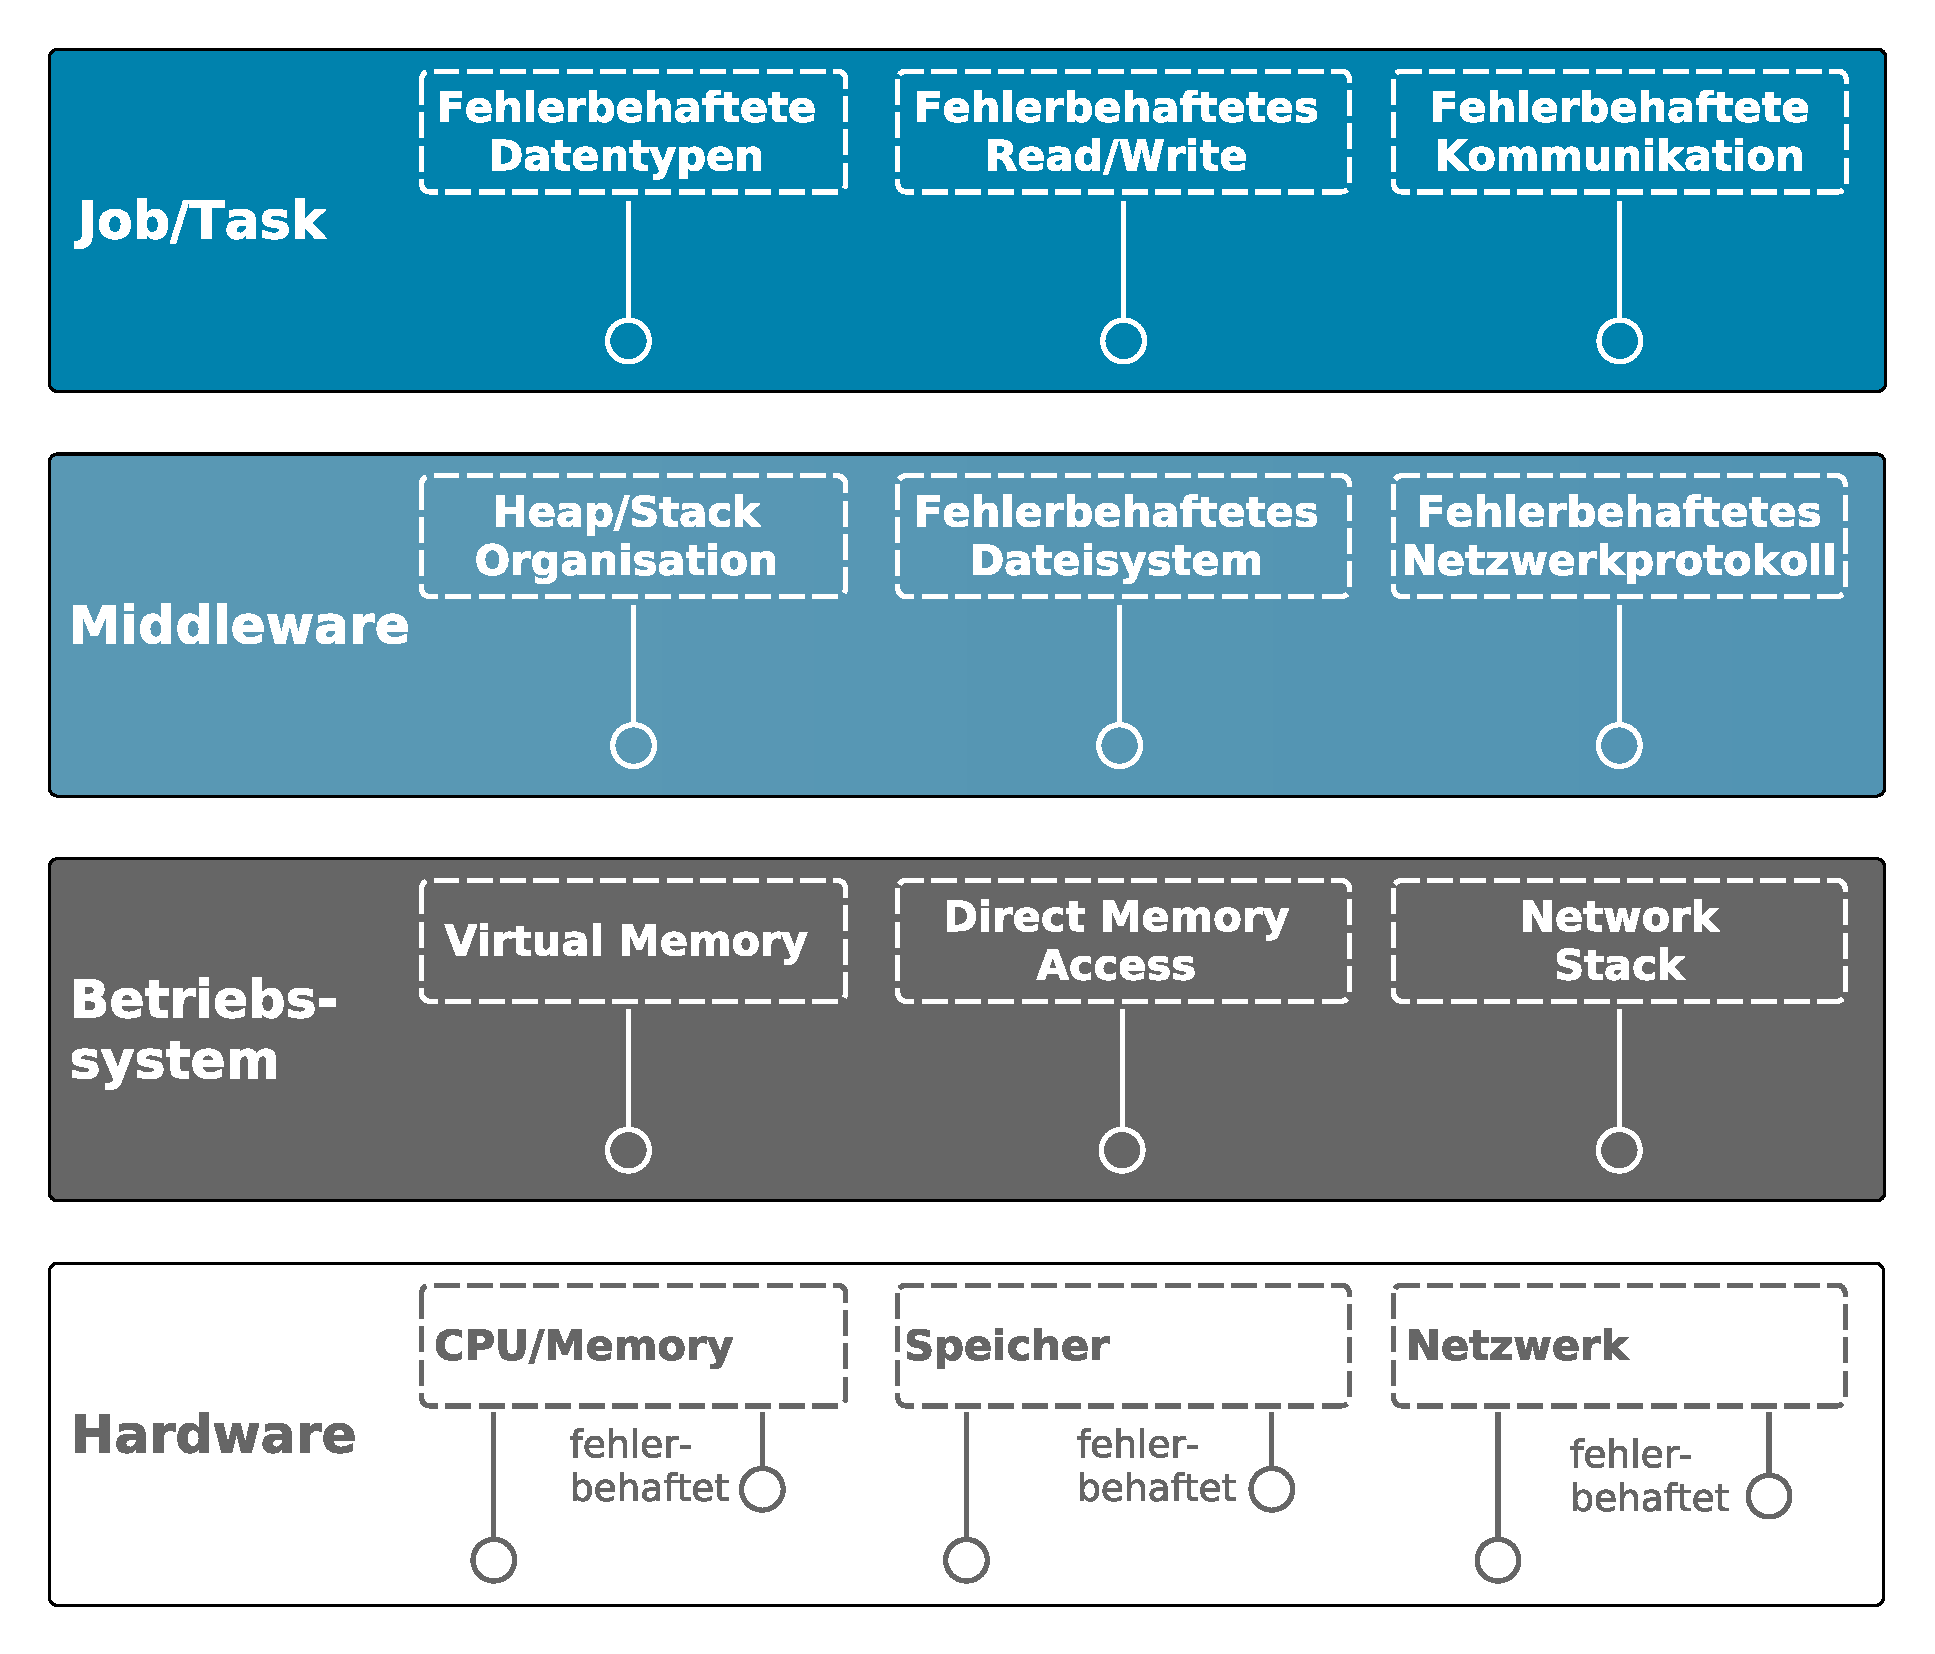
\includegraphics[scale=0.47]{graphics/AccuracyAwareness.eps}
\centering
 \caption[AccuracyAwareness: Software-Architektur]{Software-Architektur \cite{Graubner2012Energy-efficient}}
 \label{SoftwareStack}
\end{figure}

\section{Serialisierung}
Die Objektserialisierung bietet die M\"oglichkeit, Objekte auch ohne Datenbank persistent zu sichern. Dabei wird ein Objektzustand in einen Bytestrom eingepackt. Dieser kann nun problemlos \"uber ein Netzwerk transferiert und auf der anderen Seite wieder ausgepackt werden. Es wird hierbei eine Kopie des aktuellen Objektes zur\"uckgelesen. Um ein Objekt serialisierbar zu machen, muss lediglich das leere Interface \courier{java.io.Serializable} implementiert werden. Die serialisierten Objekte erhalten eine eindeutige Versionsnummer. Tr\"agt ein Objekt eine falsche Versionsnummer kann es nicht deserialisiert werden. Ist keine Nummer angegeben, so benutzt Java einen Hashwert, der sich unter anderem aus den Namen der Klassenattribute errechnet. F\"ur die Deserialisierung wird der Datenstrom eingelesen und ein Java Objekt mit dem gespeicherten Zustand erzeugt \cite{Lange}.

\section{RMI}
RMI\footnote{Remote Method Invocation} bezeichnet einen Mechanismus zur sogenannten verteilten Anwendungsprogrammierung. Vereinfacht ausgedr\"uckt erm\"oglicht es den Zugriff auf Methoden eines entfernten Java-Objekts, welches auf einer anderen Virtuellen Machine und bei Bedarf auf einem anderen vernetzten Rechner l\"auft. Die Details dieses Netzwerkverbundes bleiben dem Aufrufer verborgen, so dass die Arbeit mit verteilten Objekten sich im Prinzip kaum von der mit lokalen Objekten unterscheidet. In Abbildung \ref{RMI} ist diese Funktionsweise grafisch dargestellt.
Auf der Client-Seite nutzt Java sogenannte Stubs zur Kapselung der Daten, welche \"uber das Netzwerk verschickt werden sollen. Ein Stub implementiert das Remote-Interface und dient dem Client als Platzhalter f\"ur das Remote-Objekt. Der Stub kommuniziert \"uber die Netzwerkverbindung mit dem Skeleton auf der Serverseite. Skeletons rufen daraufhin die gew\"unschte Methode auf, \"ubergeben die Parameter und liefern das Resultat an den Client zur\"uck. Sollen komplette Objekt \"ubermitttelt werden, ist die Objekt Serialisierung erforderlich. Objekte, die als Parameter f\"ur RMI-Aufrufe dienen, m\"ussen das Interface \courier{Serializable} aus dem Package \courier{java.io} implementieren.
Die eigentliche Verbindungsaufnahme geschieht \"uber die Serveradresse und einen Bezeichner. Der Bezeichner ist notwendig damit der Namensdienst auf dem Server eine Referenz auf das entfernte Objekt zur\"uckliefern kann. Damit dies funktioniert muss sich das entfernte Objekt zuvor am Server, unter diesem Namen, beim Namensdienst registriert haben. Der RMI-Namensdienst wird \"uber statische Methoden der Klasse \courier{java.rmi.Naming} angesprochen \cite{SBoegel}.

\begin{figure}[!htb]
\centering
\begin{pspicture}(0,0)(35,20)
	\psframe[fillcolor=LLightBlue,fillstyle=solid](0,0)(35,17)
	
	\psframe[](2,17)(9.5,20)
	\psframe[fillcolor=White,fillstyle=solid](2,13.5)(9.5,17)
	\psframe[fillcolor=White,fillstyle=solid](2,7.5)(9.5,13.5)
	
	\psframe[](25.5,17)(33,20)	
	\psframe[fillcolor=White,fillstyle=solid](25.5,13.5)(33,17)
	\psframe[fillcolor=White,fillstyle=solid](25.5,7.5)(33,13.5)
	
	\psframe[fillcolor=White,fillstyle=solid](2,4)(33,7.5)
	
	\rput(28,2){\textbf{{\normalsize RMI}}}
	\rput(5.75,18.5){\textbf{{\normalsize Client}}}
	\rput(5.75,15.25){\textbf{{\normalsize Stub}}}
	\rput(5.75,10.5){\textbf{{\normalsize \parbox[c]{2cm}{Remote\\Reference\\Layer}}}}
	\rput(29.25,18.5){\textbf{{\normalsize Server}}}
	\rput(29.25,15.25){\textbf{{\normalsize Skeleton}}}
	\rput(29.25,10.5){\textbf{{\normalsize \parbox[c]{2cm}{Remote\\Reference\\Layer}}}}
	\rput(17.5,5.75){\textbf{{\normalsize Netzwerkverbindung}}}
	\rput(17.5,18.5){\textbf{Virtuelle Verbindung}}
	\psline{<-}(10,18.5)(12,18.5)
	\psline{->}(23,18.5)(25,18.5)
\end{pspicture}

 \caption[RMI Kommunikations-Architektur]{RMI Kommunikations-Architektur  \cite{SBoegel}}
 
 \label{RMI}
\end{figure}

\section{JMX}
Mittels JMX\footnote{Java Management Extensions} ist es gelungen, Java Anwendungen und Dienste über einen standardisierten Weg zu verwalten und zu \"uberwachen. Die damit entwickelte Spezifikation beschreibt eine Architektur, eine API, Design Patterns, verschiedene Verwaltungsdienste f\"ur Anwendungen sowie Monitoring Dienste f\"ur Java. Durch die Unterst\"utzung von Adaptern und Konnektoren erm\"oglicht JMX die Kommunikation zwischen verschiedenen JVM\footnote{Java Virtual Machine}. Eine Anwendung kann somit beispielsweise \"uber einen einfach implementierten HTTP-Adapter, mittels Webbrowser gesteuert werden. In Abbildung \ref{JMX} sind die verschiedenen Ebenen der JMX-Architektur dargestellt \cite{KKoehler}.\\
Die zu \"uberwachenden Resourcen befinden sich auf der Ebene Instrumentation Level. Sie werden als MBeans\footnote{Managed Bean} repräsentiert. MBeans gibt es in verschiedenen Variationen, wie beispielsweise Standard oder Dynamic MBeans. Damit der Client Zugriff auf die Resourcen bekommt, sind sogennante Agents notwendig. Diese befinden sich auf dem Agent Level\footnote{auch MBeanServer} und sprechen die Resourcen direkt an. Diese Ebene wird deshalb auch als Mittelsmann zwischen Anwendung und den MBeans bezeichnet. Das Distributed Services Level dient als Schnittstelle, um den Zugriff der Management Applikationen auf die Agents, innerhalb des Servers zu erm\"oglichen. Die verbindung wird \"uber sogenannte Connectors oder Adaptors aufgebaut. Der Connector liefert den vollen Zugang zu der MBeanServer API und kann via RMI, JMS die Verbindung herstellen. Ein Adaptor adaptiert die API auf ein anderes Protokoll wie SNMP oder auf webbasierte Oberfl\"achen wie HTML/HTTP, WML/HTTP \cite{JMXOracale}.

\begin{figure}[!htb]
\centering
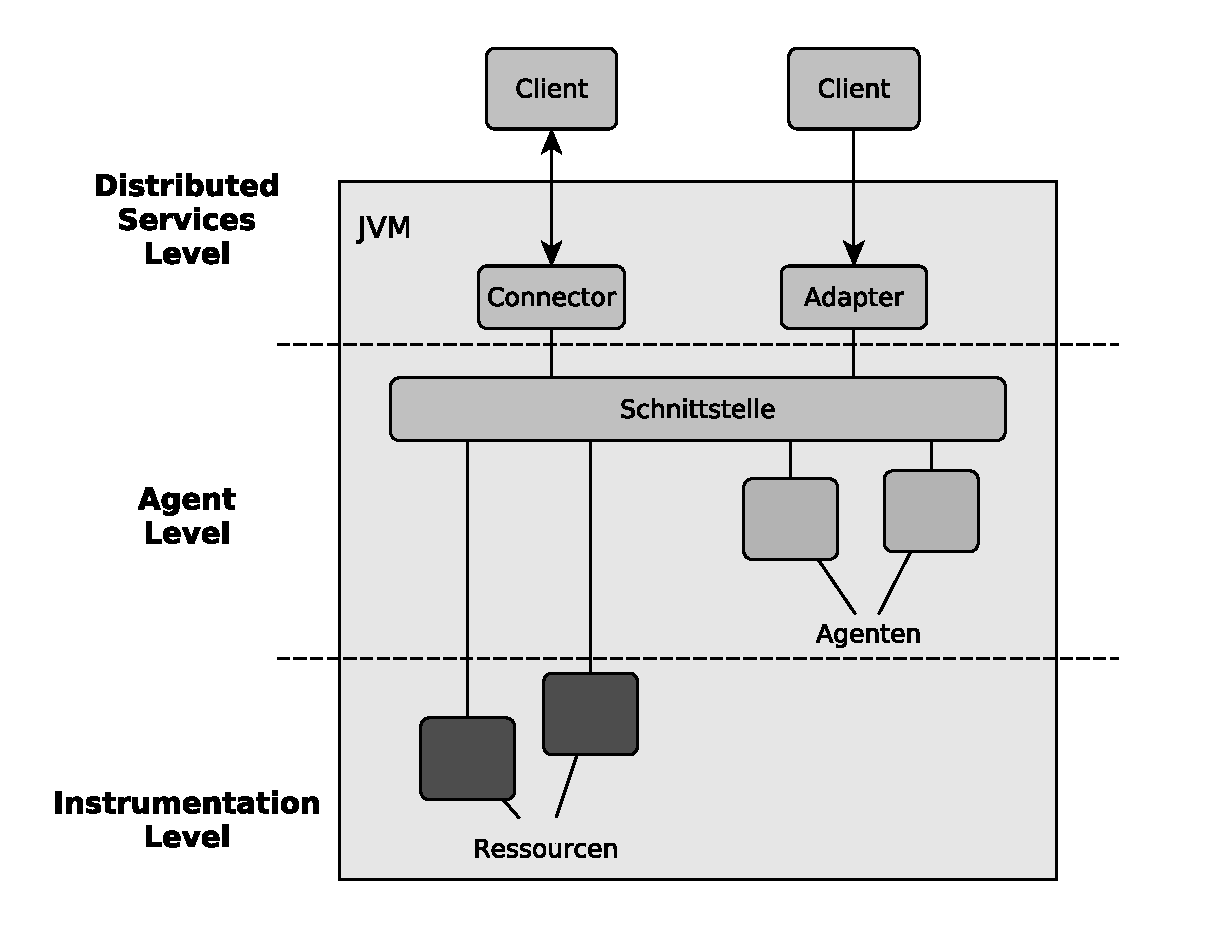
\includegraphics[scale=0.8]{graphics/JMX.eps}
 \caption[JMX-Architektur]{JMX-Architektur \cite{wikiJMX}}
 \label{JMX}
\end{figure}

\section{Jmxtools}
Die Java library Jmxtools stellt eine gro\ss e Auswahl an n\"utzlicher Zusatzfunktionalit\"at f\"ur die JMX Implementierung bereit. In dieser Arbeit wurde die Library f\"ur die Implementierung eines HTML-Clients verwendet. JMXtools bietet zu diesem Zweck einen \courier{HtmlAdaptorServer} an. Dieser erm\"oglicht es einen Zugang auf die Agent-View \"uber einen Webbrowser zu erstellen. Anschlie\ss end k\"onnen die verwalteten Ressourcen \"uber den Webbrowser verwendet werden.  

\section{Javassist}

Javassist\footnote{Java programming assistant: http://www.csg.ci.i.u-tokyo.ac.jp/$\sim$chiba/javassist/}  ist eine Java library mit deren Hilfe sich der Bytecode einer Java Anwendung leicht manipulieren oder neuer Bytecode erstellen l\"asst. Diese Eigenschaft war f\"ur die dynamische Modifikation der Fehlerwerte eine wichtige Voraussetzung.\\ Eine Java Klasse ist, sobald sie in die JVM geladen wurde, nicht mehr ohne weiteres ver\"anderbar. F\"ur diese Bachelorarbeit war es jedoch notwendig die Parameter einer Annotation zur Laufzeit modifizierbar zu halten. Da Annotationen im urspr\"unglichen Sinne, nur f\"ur den Compiler vorgesehen und deshalb auch nur zur Compilezeit ver\"anderbar sind, musste auf Bytecode-Ebene gearbeitet werden. Javassist stellt hierf\"ur die folgenden Operationen bereit.\\
Die wichtigste Klasse ist der \courier{classPool}, indem die zu manipulierenden Klassen eingef\"ugt werden m\"ussen. Anders als der JVM classloader, werden geladene Klassen durch die Javaassist API als Daten verwendbar gehalten. Klassen die in den \courier{classPool} aufgenommen werden, sind Instanzen von \courier{javassist.CtClass}. Eine \courier{CtClass} bietet zus\"atzlich zu den normalen Methoden der Class Datei die M\"oglichkeit neue Methoden, Felder und Konstruktoren der Klasse hinzuzuf\"ugen, sowie Klassenname, Superklasse und Interfaces abzu\"andern. Felder, Methoden und Konstruktoren werden durch \courier{javassist.CtField}, \courier{javassist.CtMethod}, und \courier{javassist.CtConstructor} dargestellt, welche Methoden f\"ur ihre jeweiligen Modifikationen mit sich f\"uhren \cite{JavaAssi}. Der allgemeine Modifikationsablauf ist in Abbildung \ref{Javassist} dargestellt. Hierbei wird die Ausgangsklasse \"uber die Bytecode-Manipulation um neue Aspekte, in Abbildung \ref{Javassist} die um \courier{if}-Anweisung und die \courier{@override} Annotation, erweitert. Die neu geladene Klasse enth\"alt im Anschluss beide Elemente.\\
Javassist bietet damit ausreichend Funktionionalit\"at um die gew\"unschte dynamische Regulierung umsetzen zu k\"onnen, ohne wesentliche Auswirkungen auf die Laufzeit der Anwendung zu haben. In Kapitel \ref{chp:eval} Evaluation, wurde diese Eigenschaft anhand einer Messung belegt.

\begin{figure}[!htb]
\centering
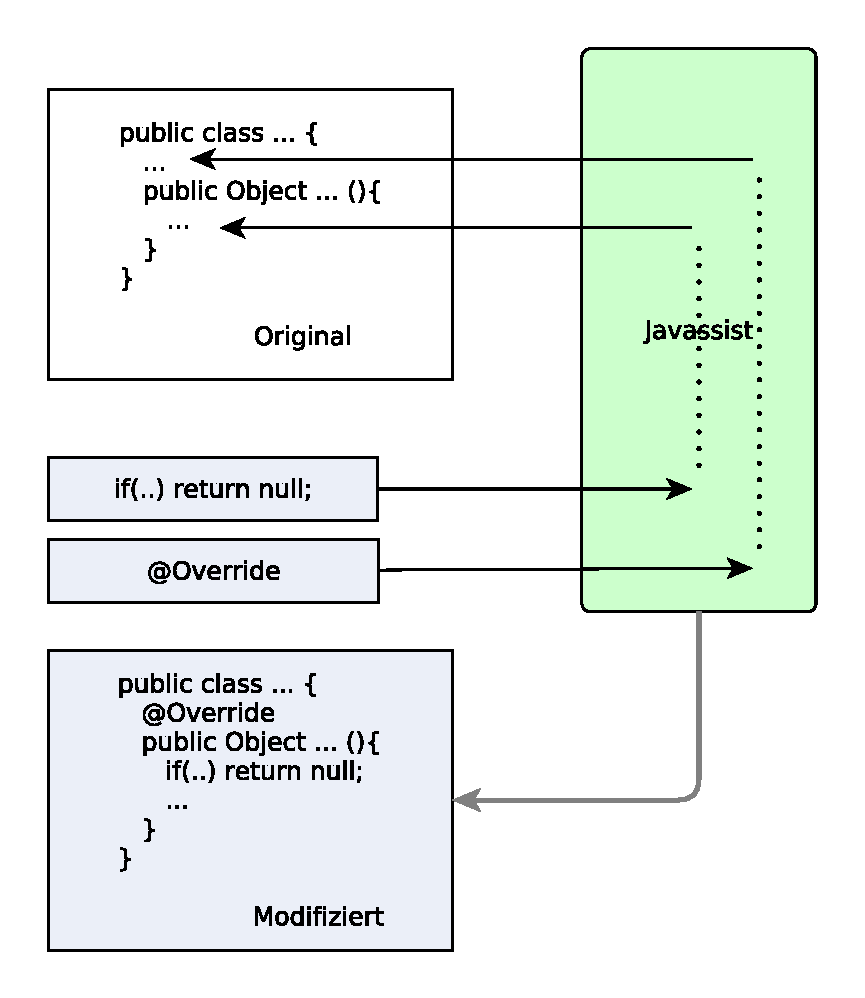
\includegraphics[scale=0.8]{graphics/javassist.eps}
 \caption[Javassist Code-Manipulation]{Code-Manipulation mit Javassist \cite{Huang:2011:SBA}}
 \label{Javassist}
\end{figure}

\section{HotSwapper}
Wie bereits beschrieben ist es durch javassist m\"oglich Klassen w\"ahrend der Laufzeit zu modifizieren und mit den neu erstellten Instanzen zu arbeiten. Sind allerdings bereits Instanzen der jeweiligen Klasse geladen, erh\"alt man die Fehlermeldung: \textit{duplicate class definition}. Um die durch javassist modifizierten Klassen respektive deren modifierzierten Bytecode f\"ur alle involvierten Objekte verwendbar zu machen, wurde \courier{javassist.util.HotSwapper}\footnote{http://www.csg.ci.i.u-tokyo.ac.jp/$\sim$chiba/javassist/html/javassist/util/HotSwapper.html} in die Implementierung eingebunden. Der \courier{Hotswapper} ben\"otigt zus\"atzlich die Einbindung der tools.jar library in den BuildPath und diverse VM-Argumente, die im Abschnitt Konfiguration im Kapitel Design erl\"autert werden. Die Funktionsweise der Klasse \courier{HotSwapper} ist in Abbildung
\ref{Swapper} grafisch dargestellt. Der neue Bytecode wird \"uber den Debugger in die Class Datei des jeweiligen Objektes eingef\"ugt und diese anschlie\ss end neu geladen. F\"ur den Ladevorgang stellt die Klasse \courier{HotSwapper} die Funktion \courier{reload} bereit. Nach dem Update des Bytecodes und dem Ladevorgang, k\"onnen alle betroffenen Klassen den neuen Code, beim Methodenaufruf ausf\"uhren.

\begin{figure}[!htb]
\centering
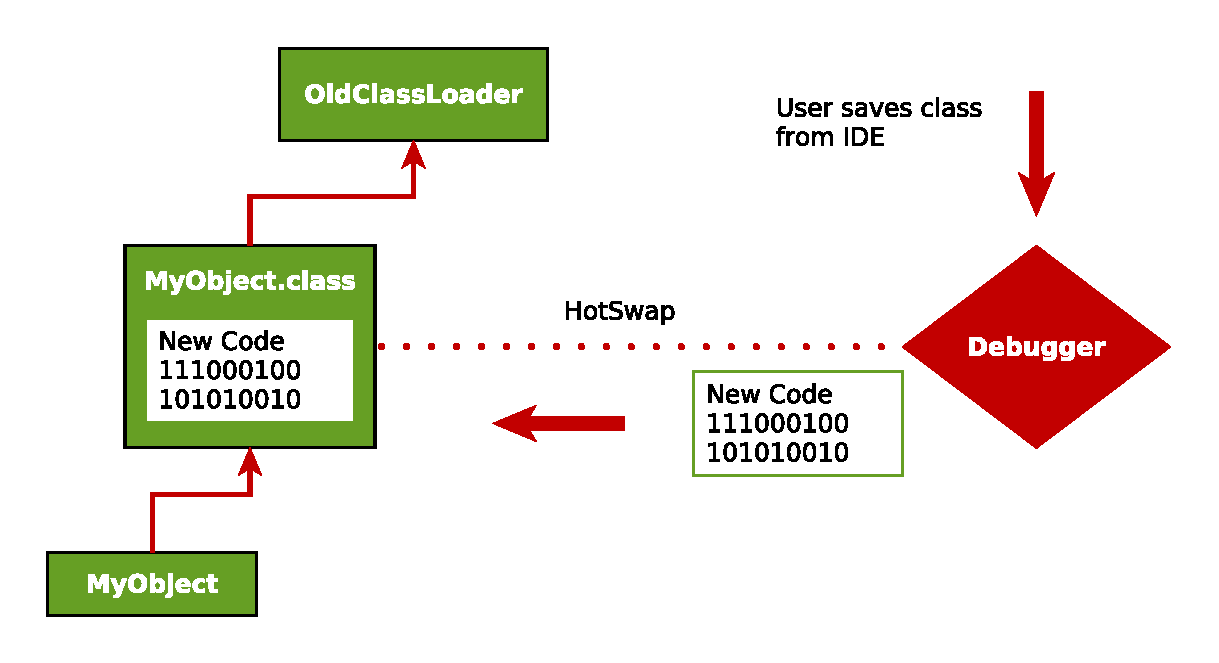
\includegraphics[scale=0.8]{graphics/HotSwapper.eps}
 \caption[Funktionsweise HotSwapper]{Funktionsweise HotSwapper \cite{HotSwapper}}
 \label{Swapper}
\end{figure}
\chapter{Verwandte Arbeiten}\vspace{1cm}
In der Informatik spielt das Thema Energieverbrauch eine besonders gro\ss e Rolle. Es existieren daher bereits viele Ans\"atze und neue Verfahren zum effizienten Umgang mit der knappen Ressource Strom. Die in diesem Kapitel diskutierten Ans\"atze fussen auf vergangenen Studien die zeigten, dass viele Programme fehlertolerant gegen\"uber geringf\"ugigen Fehlermengen sind \cite{correctness}. Verschiedene Anwendungen machen sich dieses Verhalten zunutze und erzielen mit der Differenzierung zwischen fehlerbehafteten und fehlerfreien Daten erstaunliche Ergebnisse.\\ 
Das entwickelte Programm dieser Bachelorarbeit, soll bei der Identifikation von fehlerbehafteten Daten eingesetzt werden. Konkret bearbeitet die Anwendung Datenströme, indem sie in deren Bytecode Fehlerwerte injiziert. Die Injektion geschieht \"uber die Markierung der fehlerbehafteten Streams durch eine bestimmte Annotation. Das Setzen der Fehlerwerte ist zur Laufzeit dynamisch m\"oglich, einzige Voraussetzung ist die gobale Deklaration der Streams. Die verwendete Annotation enth\"alt Parameter wie Fehlerrate, die Blockgr\"o\ss e und den Fehlertyp. Die Datensätze können somit auf ein akkurates Ma\ss {} mit Fehlern bzw. Datenverlusten injiziert werden. Letztendlich sollen dadurch Einsparungen bei der weiteren Bearbeitung erzielt und trotzdem das gew\"unschte Resultat geliefert werden. Solche Fehlerinjektionen wurden bereits in verschiedenen Anwendungen auf unterschiedlicher Weise eingef\"uhrt. 


\section{EnerJ}
Eine dieser Anwendungen, mit vergleichbarer Funktionalit\"at, ist EnerJ das eine Erweiterung der Programmiersprache Java bietet. EnerJ nutzt f\"ur die Unterscheidung zwischen fehlerfreien und fehlerbehafteten Elementen eindeutige Annotationen, welche als type-qualifier eingesetzt werden. Fehlerfreie Datentypen werden in EnerJ durch eine @Precise Annotation gekennzeichnet. Eine Annotierung präziser Datentypen ist allerdings optional, da der Default-Wert @Precise ist. Die Kennzeichnung fehlerbehafteter  Datentypen geschieht über eine @Approx Annotation. Auch in dieser Bachelorarbeit wurden Annotationen zur Fehlermarkierung eingesetzt. Ein wesentlicher Unterschied liegt in der Verwendung der Annotationen. Während EnerJ allgemeine Datentypen als approximiert oder exakt deklariert, sind die Annotationen dieser Bachelorarbeit, auschlie\ss lich auf eine variable Fehlerinjektion in Datenströmen ausgelegt.  \\
Die Korrektheit der Daten kann in EnerJ, nur bei den pr\"azisen/fehlerfreien Daten garantiert werden. Approximierte Daten haben diese Garantie nicht. Dies resultiert aus dem Grundsatz das ein Datentyp entweder pr\"azise oder approximiert sein kann. Es gibt keine verschiedenen Ebenen der Approximation, so das auch keine Garantie bzgl. der Fehlergrenzen gegeben werden kann \cite{EnerJ11}. In dieser Bachelorarbeit wurden dagegen verschiedene Ebenen eingef\"uhrt. Die Fehlerwerte der \courier{FaultInj} Annotation k\"onnen beliebig gewählt und auch zur Laufzeit angepasst werden. \\
F\"ur die Implementierung von EnerJ wurde auf das Checker Framework von Papi et al. \cite{checkerframework} zur\"uckgegriffen. Dieses erweitert das Java Typ-System und macht es um einiges vielseitiger. Es besteht aus Compiler Plug-ins sogenannten ``checkers'' und ist flexibel um weitere Compiler Plug-ins erweiterbar. Das Framework bringt einen besonderen Vorteil f\"ur die Fehlermarkierung mit sich. Indem es auch Annotationen für lokal definierte Variablen erlaubt, beitet es einen großen Handlungsspielraum. Lokale Annotationen sind ursp\"unglich nur zur Auswertung f\"ur den Compiler vorgesehen und finden aus diesem Grund in meiner Implementierung keine Anwendung. Auf die Verwendung des Checker Frameworks habe ich jedoch bewusst verzichtet, da die Verwendung dieser Technologie eine erhebliche Laufzeitverschlechterung mit sich bringt.

\section{Green-Framework}
Ein weiterer \"ahnlicher Ansatz findet sich im Green-Framework von Woongki Baek und Trishul M. Chilimbi. Diese Anwendung bietet ein flexibles Framework, welches versucht un\"otige Genauigkeiten durch Approximationen zu kompensieren. Das Framework fokusiert sich dabei allerdings auf Approximationen f\"ur Schleifen und Funktionen, wodurch es sich von meiner Implementierung bereits abgrenzt. Jedoch bietet es ebenfalls verschiedene Ebenen der Fehlerinjektion. Der Entwickler hat die M\"oglichkeit einen maximalen Verlust bez\"uglich der Anforderungen/QoS\footnote{Quality of Service} anzugeben. Das Green-Framework liefert im Anschluss eine Auswertung, inwieweit die Anwendung diesen Anforderung gen\"ugen wird. Um approximierte Funktionen nutzen zu k\"onnen, muss der Entwickler diese zus\"atzlich bereitstellen. Schleifen k\"onnen beispielsweise durch weniger Iterationen approximiert werden. Am Ende erstellt der Green Compiler, auf Grundlage eines generierten QoS-Models mit dem ursp\"unglichen Programm, eine energieeffizientere Anwendung mit den approximierten Funktionen \cite{green}. 

\section{Probabilistic Accuracy Bounds}
Die Arbeit von Martin Rinard, ``Probabilistic Accuracy Bounds for Fault-Tolerant
Computations that Discard Tasks'' besch\"aftigt sich ebenfalls mit einer Methode die es erm\"oglicht,  Berechnungen mit Datenfehlern auszuführen und dennoch einen vern\"unftigen Output zu erzeugen. \\ 
Die Berechnungen werden bei diesem Ansatz in einzelne Tasks eingeteilt. Bei der Ausf\"uhrung werden Tasks, bei denen Fehler bzw. St\"orungen vorhanden waren, einfach verworfen. Die fehlerfreien Tasks setzen die Berechnung bis zum Ende fort. Das Modell verwendet als Grundlage zuf\"allige Ausf\"uhrungen eines Programms mit unterschliedlichen Task-Fehlerraten. Anhand dieser Ausführungen wird ein quantitatives, probabilistisches Modell erstellt. Das Modell charakterisiert die Verzerrung des Outputs. Durch die somit definierten Grenzen, leistet die Anwendung trotz Fehlern einen qualitativen Output. Weiterhin ist die Erstellung eines Timing-Modells\footnote{Ausf\"uhrungszeit als Funktion über Task Fehlerraten} vorgesehen. Die Kombination der beiden Modelle erlaubt es die Genauigkeit der Ausf\"uhrung zu reduzieren. Die Fehlerinjektion wird bei diesem Ansatz durch eine Injektion mit fehlerhaften Tasks vogenommen. Dadurch lässt sich Ausf\"uhrungszeit sparen, w\"ahrend die Abweichung der Berechung innerhalb akzeptabler Grenzen liegt \cite{Rinard06}. 

\section{Loop Perforation}
Eine weitere Technik, um die Genauigkeit einer Anwendung zu reduzieren und damit einen Leistungszuwachs zu erzielen, ist die ``loop perforation'' von Stelios Sidiroglou-Douskos  et al.\\
Diese Anwendung versucht analog zum Green-Framework, eine bessere Performance durch effizientere Berechnungen in Schleifen zu erzielen. Im kern wird versucht die Anzahl der Iterationen von Schleifen zu reduzieren, um somit einen geringeren Rechenaufwand zu erhalten. Dieser Vorgang wird ``Perforierung'' genannt. Das Verfahren filtert f\"ur die Unterscheidung von fehlerfreien und fehlerbehafteten Daten zun\"achst die kritischen Schleifen heraus, dieser Vorgang nennt sich ``Criticality Testing''. Alle kritischen Schleifen, sind Schleifen die durch die Perforierung einen Schaden verursachen. Alle nicht kritischen Schleifen k\"onnen durch die Perforierung einen erheblichen Effizientzanstieg, bei einer weiterhin akzeptablen Genauigkeit erzielen. Die zweite Phase ist der ``Perforation Space Exploration'' Algorithmus. Alle nicht kritischen Schleifen werden in dieser Phase verarbeitet, indem versucht wird sie optimal zu kombinieren. Dadurch entsteht eine Menge von Pareto-optimalen\footnote{Zustand, in dem ein Individuum nicht besser gestellt werden kann} Varianten mit bestm\"oglicher Perfomance, bei einem bestimmten Genauigkeitsverlust \cite{loopPerforation}. Die Anwendung fokusiert sich im Gegensatz zu meiner Implementierung auf Schleifen. Die Fehlerinjektion beginnt beim Criticality Testing und wird anschlie\ss end algorithmisch optimiert. Die Optimierung wird grunds\"atzlich durch eine Reduzierung von Schleifeniterationen vorgenommen. Die Anwendung dieser Bachelorarbeit bietet bezieht sich ausschlie\ss lich auf Datenströme. Zusätzlich wird vielseitigerer Injektionsmechanismus mit diversen Fehlertypen und variabel anpassbarer Fehlerrate angeboten. 
\chapter{Design}\vspace{1cm}
Das Kapitel Design beschreibt zunächst die Problemstellung der zugrundeliegenden Arbeit. Zu diesem Zweck wird die bestehende Ausgangssituation aufgezeigt sowie eine kurze Einführung hinsichtlich der Funktionsweise der Anwendung gegeben. Ein Anwendungsfall beschreibt infolge einer dargestellten Benutzerinteraktion die zur Verfügung gestellten Operationen. Im Hauptteil werden die wichtigsten Klassen bezüglich deren Abhängigkeiten und Funktionsweisen vorgestellt. Für die Visualisierung dieser Eigenschaften wurde die graphische Modellierungssprache UML  eingesetzt. Es werden allgemeine Designentscheidungen diskutiert und abschlie\ss end ein Gesamt\"uberblick anhand eines sequentiellen Programmablaufs gegeben.
%
\section{Motivation und Zielsetzung}

Es wurde bereits in den vorherigen Kapiteln erwähnt, dass Energie in der Zukunft eine immer knapper werdende Ressource sein wird. Gerade in der Informatik steigt der Energiekonsum aufgrund neuer Technologien und Online-Services stetig an \cite{Kommey}. Das f\"ur diese Bachelorarbeit entwickelte Programm ist Bestandteil einer Forschung, welche versucht dieses Problem zu l\"osen, indem es mit Hilfe des Paradigmas Accuracy Aware eine energiebewusste Programmierung erm\"oglicht. \\
Die Zielsetzungen waren:
\begin{itemize}
	\item die Fehlerinjektion minimal-invasiv, d.h. mit möglichst wenig Änderungen im Code vornehmen zu müssen.   
	\item Nur einen minimalen Overhead erzeugen, um die Verwendung für große verteilte Systeme (z.B. Hadoop), bei denen neben der Fehlerinjektion zugleich Energiemessungen vorgenommen werden können, zu ermöglichen.
	\item Alle Arten von Datenströmen, wie FileIO oder Network, sollten berücksichtigt werden, weil für ``Accuracy Awareness'' sowohl modifizierte Disk- als auch Network-Hardware simuliert werden soll.
	\item Eine dynamische Regulierung der Fehlerwerte zur Laufzeit. Dem Client sollte es somit m\"oglich sein Fehlerwerte, welche vorher im Programmcode festgelegt wurden, im laufenden Programm modifizieren zu k\"onnen.
\end{itemize}

Das Programm verwendet zun\"achst gew\"ohnliche Streams um Daten einzulesen. Diese werden anschlie\ss end ``verpackt'' und \"uber verschiedene Logiken mit Fehlerwerten injiziert. Danach werden die injizierten Daten für die weitere Verwendung ausgegeben. Die Fehlerinjektion wird über eine Markierung der betroffenen Streams durch Java Annotations\footnote{Metadaten} im Quelltext eingeleitet. Jeder markierte Stream wird somit als fehlerbehaftet gekennzeichnet und bekommt von Beginn an Fehlerwerte zugewiesen. Für die Markierungen wurde eine selbstdefinierte Annotation mit dem Namen \courier{FaultInj} verwendet. Die Fehlerwerte sind durch die vier Parameter ID, Fehlerrate, Fehlertyp und die Gr\"o\ss e eines fehlerbehafteten Datenblocks definiert. Ziel der Fehlerinjektion ist es, die eingelesen Daten mittels diesen konkreten Fehlerwerten und diversen Injektionsstrategien manipulieren zu k\"onnen. F\"ur die Fehlerinjektion war es zusätzlich notwendig, auch mehrere Markierungen/Annotationen mit verschiedenen Werten f\"ur einen Stream definieren zu k\"onnen. 

\section{Benutzerinteraktion}
Die Benutzerinteraktion wurde sehr übersichtlich gestaltet, um den Client eine m\"oglichst kompakte, intuitive Bedienbarkeit zur Verfügung zu stellen. F\"ur den Anwender wurde deshalb eine Schnittstelle mit dem MBean Server kreiert (Siehe dazu Abschnitt \ref{controller}), welche ausschlie\ss lich vier unterschiedliche Funktionalitäten anbietet. \\
In Abbildung \ref{AnFallDia} ist diese Benutzerinteraktion als Anwendungsfalldiagramm bzw. Nutzfalldiagramm dargestellt. Die ersten beiden Operationen der Anwendung mit ähnlicher Funktionalität, geben alle Fehlerwerte respektive die ID's der annotierten Streams zurück. Dies ist insbesondere von Vorteil, wenn später die Fehlerwerte geändert werden sollen und die eindeutige ID des Streams nicht bekannt ist. \\
Um die Fehlerwerte der einzelnen Streams ändern zu können, gibt es eine Methode die in Abbildung \ref{AnFallDia} unter ``Fehlerwerte \"andern'' zu finden ist. Die Änderungsmöglichkeiten umfassen die Fehlerrate, Fehlertyp und die grö\ss e des Datenblocks. Die ID dient zur Zuordnung der Fehlerwerte und kann ausschlie\ss lich im Programmcode ver\"andert werden.\\
Die wichtigste Funktion hat den Namen \courier{runInjection} und ist in Abbildung \ref{AnFallDia} als ``Injektion durchführen'' dargestellt. Für diese Funktion lassen sich zwei Varianten auswählen. Die erste Variante ist für eine Dateiinjektion definiert und benötigt lediglich den Dateipfad. Die zweite Variante verlangt einen Java \courier{InputStream} um allgemeine Datenströme zu verarbeiten. Nach dem Laden der Daten wird durch diese Funktion die eigentliche Fehlerinjektion und die Datenausgabe veranlasst.\\
Für die Datenausgabe sind ebenfalls zwei Wahlmöglichkeiten vorhanden, deren genaue Differenzierung im weiteren Verlauf dieses Kapitels erläutert wird.

\begin{figure}[!htb]
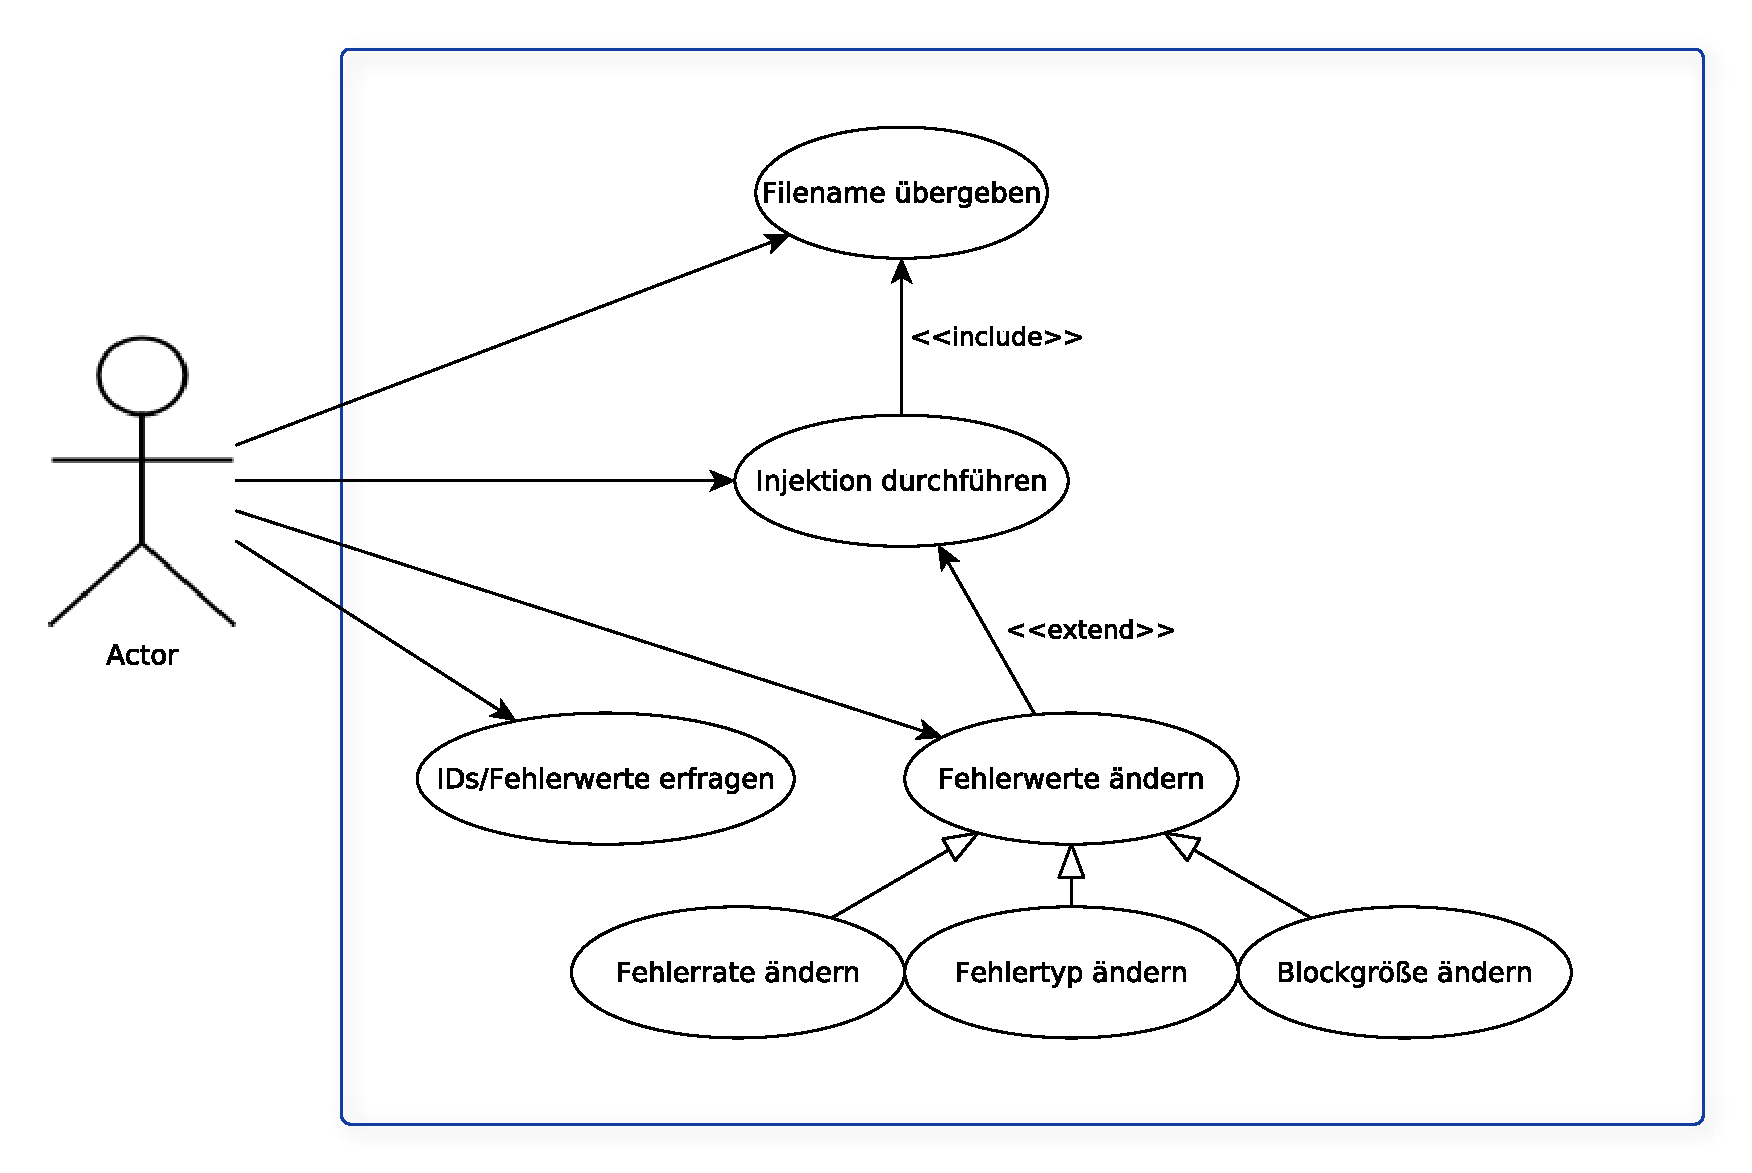
\includegraphics[scale=0.55]{graphics/Anwendungsfalldiagramm.eps}
\centering
 \caption[Anwendungsfalldiagramm]{Anwendungsfalldiagramm}
 \label{AnFallDia}
\end{figure}


\section{Klassendesign \& -abhängigkeiten}
%
Die Klassenhierarchie der zugrunde liegenden Anwendung st\"utzt sich auf den folgenden vier S\"aulen, welche das Grundgerüst bzw. die Hauptfunktionalität der Applikation bilden. Ein wesentliches Ziel war es, die Anforderungen der Modularit\"at zu erf\"ullen. Die Anwendung sollte für eventuelle Erweiterungen m\"oglichst flexibel und gut strukturiert bleiben.
%
	\begin{itemize}
		\item StreamProcesser : Einlesen und Ausgabe der Daten, Start der Fehlerinjektion
		\item InjectionStrategy : Oberklasse der Injektionsstrategien
		\item AddRunTimeAnnotation : Dynamische Modifikation der Annotationen
		\item Controller : Steurerung aller Funktionen
	\end{itemize}	 
%
\subsection{StreamProcessor}

Der \courier{StreamProcessor} ist das Herzst\"uck der Anwendung. Alle Daten die es zu manipulieren gilt, werden an diese Klasse übergeben. Die für das Einlesen der Daten notwenigen Streams sind in der Klassendefinition als globale Variablen vorgesehen. Dies bedeutet auch, dass die Fehlermarkierungen durch die \courier{FaultInj} bzw. mehrere Markierungen durch eine \courier{FaultInjects} Annotation, ausschlie\ss lich global vorgenommen werden können.\\ 
Der \courier{StreamProcessor} zerlegt einen Datenstream in einzelne Bytes, um sie anschlie\ss end der Klasse \courier{Context} zu übergeben. Die Klasse \courier{Context} verwaltet die Daten zusammen mit deren Fehlerwerte, falls jene definiert wurden. Die Implementierung erlaubt es an dieser Stelle auch mehrere Datens\"atze verschiedener Streams durch ein \courier{Context} Objekt verwalten zu lassen. Für jeden Datensatz wird eine eindeutige ID zur Unterscheidung festgelegt. Einzige Prämisse für die Nutzung dieser Datenverwaltung ist die Serialisierbarkeit der Daten, um einen Netzwerktransfer zu erm\"oglichen.\\
Nach dem Einlesevorgang wird über den \courier{StreamProcessor} die Fehlerinjektion veranlasst. Bereits während des Einlesens wurden für jeden Datensatz, anhand der ID des markierten Streams, die Fehlerwerte registriert. Der \courier{StreamProcessor }startet nun die Fehlerinjektion über seine Instanz der Klasse \courier{Context}. Diese bestimmt anhand des Fehlertyps die notwendige Injektions-Strategie. Ist für einen Datensatz kein Strategie vorhanden bleibt dieser unberührt und eine Fehlermeldung wird ausgegeben. Für die konkrete Fehlerinjektion wurde ein Strategy Pattern in leicht abgewandelter Form verwendet. \\
Die aktuelle Implementierung sieht nach der Fehlerinjektion die Datenausgabe in eine Datei vor. Zu diesem Zweck wurde eine innere Klasse \courier{Reducer} implementiert. Sie ist f\"ur die Erstellung der neuen Dateien zust\"andig und bietet hierfür zwei verschiedene Ausgabevarianten an. Per Default wird ein \courier{FileChannel} für die Ausgabe verwendet. Durch eine zusätzliche Funktion kann der Ausgabestream vom Client, zu einem \courier{ObjectOutputStream} geändert werden. Dadurch wird eine persistente Objektspeicherung ermöglicht. Nach diesem Schritt wird durch alle Datens\"atze iteriert und die Daten in die neuen Dateien geschrieben. Diese Struktur ist in Abbildung \ref{FileProcessorUML} als UML-Klassendiagramm dargestellt.

\begin{figure}[!htb] 
\centering
		\umlDiagram[box=,border,sizeX=12cm,sizeY=10cm,ref=pack]{		
			\umlClass[pos=\umlTop{pack}, stereotype=Class, posDelta={0, -10},
				refpoint=t]{StreamProcessor}{}{}
			\umlClass[pos=\umlTop{pack}, stereotype=Class, posDelta={0, -1},
				refpoint=t]{Context}{}{}
			\umlClass[pos=\umlTopRight{pack}, stereotype=Abstract Class, posDelta={-6,-1},
				refpoint=t]{InjectionStrategy}{}{}	
			\umlClass[pos=\umlLeft{pack}, stereotype=Class, posDelta={4, 2},
				refpoint=t]{Reducer}{}{}	
			\umlClass[pos=\umlRight{pack}, stereotype=Annotation, posDelta={-5, 2},
				refpoint=t]{FaultInj}{}{}
			\umlClass[pos=\umlBottom{pack}, stereotype=Annotation, posDelta={0, 6},
				refpoint=t]{FaultInjects}{}{}																	\umlInner{Reducer}{StreamProcessor}
			\umlInstance{StreamProcessor}{FaultInj}	
			\umlInstance{StreamProcessor}{FaultInjects}
			\umlInstance{StreamProcessor}{Context}
			\umlInstance{Context}{InjectionStrategy}									
		}% End of diagram
%		\captionsetup{list=false}
	\caption{UML StreamProcessor}
 	\label{FileProcessorUML}
\end{figure}

\subsection*{Exkurs: Klasse Context}

Bisher wurde häufig die Klasse \courier{Context} erwähnt, welche die eingelesenen Daten verwaltet und  Fehler in die enthaltenen Datensätze einbaut. Um diese Aufgabe zu erfüllen, muss die Klasse \courier{Context} zunächst für jeden Datensatz die erforderliche Injektionslogik bestimmen. Die Injektionslogiken wurden durch eine Form des Strategy Patterns \cite{GammaEtAl00} in die Implementierung integriert.\\
Die Klasse \courier{Context} trifft die Auswahl der konkreten Injektionsstrategie anhand des Fehlertyps des jeweiligen Datensatzes. Eine abstrakte Klasse repräsentiert die allgemeinste Strategie. Sie kann flexibel von den beschriebenen Logiken in den folgenden Abschnitten erweitert/überschrieben werden. Die verschiedenen Strategien sind als einzelne Module definiert, die problemlos durch neue Klassen erg\"anzt werden können. Wenn die richtige Strategie gefunden wurde, kann die Injektion mit den entsprechenden Fehlerwerten gestartet werden.
%
\subsection{Fehlerwerte}
Fehlerwerte sind im Programmcode als Annotationen darstellt. Ein Stream kann dabei auch mit mehreren Annotationen versehen werden. Der Fehlerwert besteht immer aus den folgenden vier Komponenten:

\begin{itemize}
	\item ID: Die ID ist ein eindeutiger Wert zur Unterscheidung bzw. Identifikation der einzelnen Streams. Soll ein Fehlerwert dynamisch ver\"andert werden, wird dieser \"uber die ID angesprochen. Sie wird dementsprechend in der Implementierung gesetzt und kann w\"ahrend der Laufzeit nicht ver\"andert werden.
	\item Type: Der Fehlertyp wird \"uber den Parameter \courier{type} angesprochen. Er repr\"asentiert die Fehlerlogik die angewendet werden soll. Als m\"ogliche Typen stehen in dieser Version der Anwendung RANDOM, LOSS, ZERO, BITFLIP, BITFLIPB, NONE zu Verf\"ugung. Auf deren genauere Bedeutung wird in den folgenden Abschnitten der konkreten Logiken eingegangen.
	\item Rate: Die Fehlerrate ist eine Gleitkommazahl doppelter Genauigkeit und liegt zwischen 0 und 1. Sie gibt die Wahrscheinlichkeit der Injektion eines Blocks oder Bits an. Die Werte stehen für 0\% bis 100\% und flie\ss en in die Berechnung einer Zufallsfunktion ein. Diese  erstellt auf Grundlage der statischen Methode \courier{random} aus der Klasse \courier{Math} einen Zufallswert und setzt diesen in Relation zu der Fehlerrate. Das Ergbnis der Berechnung liefert die Entscheidung über die Injektion eines Blocks oder Bits, abhängig von der konkreten Strategie. Bei einer Fehlerrate von 1 würden demnach alle Blöcke oder Bits injiziert werden.
	\item Blocksize: Die Blockgr\"o\ss e bestimmt die Anzahl der zu injizierenden Bytes, die in einen Block gepackt werden sollen. Bis auf die einfache Bitflip Strategie sind alle Injektionsstrategien auf den Blocksize Parameter angewiesen. Die eben beschriebene Zufallsfunktion arbeitet f\"ur diese Logiken auf der Blockebene. Das hei\ss t die Zufallsentscheidung der Injektion wird nicht f\"ur einzelne Bytes, sondern f\"ur den gesamten Block getroffen.
\end{itemize}

\label{strats}
\subsection{Injektions-Strategie}

Die abstrakte Klasse \courier{InjectionStrategy} wurde als Oberklasse für alle konkreten Strategien definiert. Sie enthält keine eigene Injektionslogik, fordert aber die Implementierung einer Injektionslogik von ihren Unterklassen. Sie stellt ebenso die Zufallsfunktion als auch die Fehlerwerte für ihre Unterklassen zur Verfügung. In Abbildung \ref{StrategyUML} wurde dieses Muster, zuzügliche der Verbindung zur Klasse \courier{Context}, modelliert.

\begin{figure}[!htb] 
\centering
		\umlDiagram[box=,border,sizeX=12cm,sizeY=14cm,ref=pack]{	
			\umlClass[pos=\umlTop{pack}, stereotype=Class, posDelta={0, -1},
				refpoint=t]{Context}{}{}	
			\umlClass[pos=\umlTop{pack}, stereotype=Abstract Class, posDelta={0, -8},
				refpoint=t]{InjectionStrategy}{
					\umlAttribute[visibility=\# , type=FaultValue{[]}]{faults}				
				}{
					\umlMethod[visibility=+, type=void]{\textit{runInjection}}{}
					\umlMethod[visibility=\# , type=boolean]{isInject}{double}				
				}
			\umlClass[pos=\umlLeft{pack}, stereotype=Class, posDelta={5.5, 0},
				refpoint=t]{StrategyBitflip}{}{
					\umlMethod[visibility=+, type=void]{runInjection}{}				
				}
			\umlClass[pos=\umlRight{pack}, stereotype=Class, posDelta={-5.5, 0},
				refpoint=t]{StrategyBitflipB}{}{
					\umlMethod[visibility=+, type=void]{runInjection}{}					
				}	
			\umlClass[pos=\umlBottomLeft{pack}, stereotype=Class, posDelta={7, 7},
				refpoint=t]{StrategyLoss}{}{
					\umlMethod[visibility=+, type=void]{runInjection}{}					
				}	
			\umlClass[pos=\umlBottomRight{pack}, stereotype=Class, posDelta={-7, 7},
				refpoint=t]{StrategyRandom}{}{
					\umlMethod[visibility=+, type=void]{runInjection}{}					
				}
			\umlClass[pos=\umlBottom{pack}, stereotype=Class, posDelta={0, 7},
				refpoint=t]{...}{}{
					\umlMethod[visibility=+, type=void]{runInjection}{}					
				}				
			\umlInstance{Context}{InjectionStrategy}									
			\umlSubclass{InjectionStrategy}{StrategyBitflip}	
			\umlSubclass{InjectionStrategy}{StrategyBitflipB}
			\umlSubclass{InjectionStrategy}{...}	
			\umlSubclass{InjectionStrategy}{StrategyLoss}
			\umlSubclass{InjectionStrategy}{StrategyRandom}											
		}% End of diagram
	%	\captionsetup{list=false}
	\caption[UML Strategy Pattern]{UML Strategy Pattern}
 	\label{StrategyUML}
\end{figure}



\subsubsection{Strategie Bitflip}

Die erste Strategie tr\"agt den Namen Bitflip und ist in der Regel das aufwendigste Verfahren. Grund daf\"ur ist die individuelle Verwendung der Zufallsfunktion f\"ur jedes einzelne Bit. Auch die Datenmanipulation muss, auf Grundlage des Resultats dieser Funktion entsprechend h\"aufig ausgef\"uhrt werden. Wie der Name Bitflip schon verrät, werden bei dieser Strategie Bits lediglich umgedreht\footnote{flip: 0 zu 1 und 1 zu 0}. Im folgenden Beispiel wurden durch die Zufallsfunktion, die Bits an den Positionen 3,4 und 7 ausgew\"ahlt und entsprechend injiziert. \\

\psline[linecolor=red,linewidth=.1cm,
doublesep=1.5pt]{->}(5.2,1.5)(5.2,0)
\psline[linecolor=red,linewidth=.1cm,
doublesep=1.5pt]{->}(6.8,1.5)(6.8,0)
\psline[linecolor=red,linewidth=.1cm,
doublesep=1.5pt]{->}(11.5,1.5)(11.5,0)
\psline[linecolor=red,linewidth=.1cm,
doublesep=1.5pt]{->}(25.5,1.5)(25.5,0)
\psline[linecolor=red,linewidth=.1cm,
doublesep=1.5pt]{->}(27.1,1.5)(27.1,0)
\psline[linecolor=red,linewidth=.1cm,
doublesep=1.5pt]{->}(31.8,1.5)(31.8,0)


$\dots$
\begin{tabular}{|c|c|c|c|c|c|c|c|}
\hline
0 & 1 & 0 & 0 & 0 & 1 & 1 & 1 \\\hline
\end{tabular}
$\dots$
\psline[linewidth=.1cm]{->}(0.5,0)(4,0)
\hspace{2cm}$\dots$
\begin{tabular}{|c|c|c|c|c|c|c|c|}
\hline
0 & 1 & 1 & 1 & 0 & 1 & 0 & 1 \\\hline
\end{tabular}
$\dots$

\subsubsection{Strategie BitflipB}

Diese Strategie funktioniert analog zum normalen Bitflip. Einzige Ausnahmen sind die Bearbeitung ganzer Bytes statt einzelner Bits sowie die Möglichkeit der Blockverarbeitung. Die Zufallsfunktion entscheidet diesmal individuell f\"ur jeden Block \"uber dessen Injektion. Wird ein Block zur Injektion ausgew\"ahlt, werden s\"amtliche Bits der darin enthaltenen Bytes gedreht. Wird der Block nicht ausgew\"ahlt, bleiben die Bytes komplett erhalten.\\

$\dots$
\begin{tabular}{|c|c|c|c|c|c|c|c|}
\hline
0 & 1 & 0 & 0 & 0 & 1 & 1 & 1 \\\hline
\end{tabular}
$\dots$
\psline[linewidth=.1cm]{->}(0.5,0)(4,0)
\hspace{2cm}$\dots$
\begin{tabular}{|c|c|c|c|c|c|c|c|}
\hline
1 & 0 & 1 & 1 & 1 & 0 & 0 & 0 \\\hline
\end{tabular}
$\dots$


\subsubsection{Strategie Loss}
Loss ist eine Strategie die das Löschen von ganzen Byte-Blöcken ermöglicht. Wird ein Block im Datensatz zur Injektion ausgewählt, werden sämtliche Bytes des Blocks entfernt. Im Beispiel wird ein Block mit einer Größe von zwei aus dem Datensatz ausgewählt und beide Bytes entfernt.\\

\psbrace[linecolor=red,fillcolor=red, rot=-90,nodesepA=-2pt, nodesepB=17pt](1,2.5)(1,-0.3){injiziert}
\phantom{$\dots$}
\begin{tabular}{|c|c|c|c|c|c|c|c|}
\hline
0 & 1 & 0 & 0 & 0 & 1 & 1 & 1 \\\hline
0 & 0 & 0 & 0 & 0 & 0 & 0 & 0 \\\hline
1 & 1 & 1 & 0 & 0 & 1 & 1 & 1 \\\hline
\end{tabular}
$\dots$
\psline[linewidth=.1cm]{->}(0.5,0)(4,0)
\hspace{2cm}$\dots$
\begin{tabular}{|c|c|c|c|c|c|c|c|}
\hline
1 & 1 & 1 & 0 & 0 & 1 & 1 & 1 \\\hline
\end{tabular}
$\dots$

\subsubsection{Strategie Random}
Die Strategie Random verfügt über einen weiteren Zufallsgenerator. Dieser erstellt für die injizierten Blöcke zufällige Bytes. Die alten Bytes des jeweiligen Blocks werden im Anschluss durch die neu generierten Bytes ersetzt. \\

$\dots$
\begin{tabular}{|c|c|c|c|c|c|c|c|}
\hline
0 & 1 & 0 & 0 & 0 & 1 & 1 & 1 \\\hline
\end{tabular}
$\dots$
\psline[linewidth=.1cm]{->}(0.5,0)(4,0)
\hspace{2cm}$\dots$
\begin{tabular}{|c|c|c|c|c|c|c|c|}
\hline
0 & 1 & 1 & 0 & 1 & 0 & 0 & 1 \\\hline
\end{tabular}
$\dots$


\subsubsection{StrategyZero}
Diese Strategie funktioniert analog zur Random Strategie. Es werden diesmal allerdings Null-Bytes, statt zufällige Bytes für die Ersetzungen im injizierten Block verwendet. Das folgende Beispiel zeigt ein Byte das bei einer Blockgröße von eins ausgewählt und durch die Zero Strategie injiziert wurde.\\

$\dots$
\begin{tabular}{|c|c|c|c|c|c|c|c|}
\hline
0 & 1 & 0 & 0 & 0 & 1 & 1 & 1 \\\hline
\end{tabular}
$\dots$
\psline[linewidth=.1cm]{->}(0.5,0)(4,0)
\hspace{2cm}$\dots$
\begin{tabular}{|c|c|c|c|c|c|c|c|}
\hline
0 & 0 & 0 & 0 & 0 & 0 & 0 & 0 \\\hline
\end{tabular}
$\dots$


\subsubsection{Strategie None}
Soll keine Injektion ausgef\"uhrt werden, besteht die M\"oglichkeit die Fehlerrate auf 0 oder den Fehlertyp auf NONE zu setzen. Beide Varianten liefern als Resultat die Ausgangsdaten zur\"uck. Einfaches Entfernen des Fehlertyps reicht nicht aus und würde zu einer Fehlermeldung führen.
%
\subsection{Dynamische Konfiguration}

Die Klasse \courier{AddRunTimeAnnotation} ist f\"ur die dynamische Anpassung der Fehlerwerte zur Laufzeit verantwortlich. Annotationen sind urspr\"unglich nur Metainformationen, die im Quelltext eines Programmes notiert werden und zusätzlich semantische Informationen bereit stellen. Problematisch an der Verwendung von Annotationen ist die Tatsache, dass sich diese nicht ohne weiteres dynamisch verändern lassen. Aus diesem Grund wurden verschiedene L\"osungswege getestet und schlie\ss lich eine Manipulation auf Bytecode-Ebene durchgef\"uhrt. Zu diesem Zweck wurde sich die Funktionalit\"at der Bibliotheken Javassist und Tools zunutze gemacht, welche im Kapitel Grundlagen bzw. deren genaue Konfiguration im Abschnitt Voraussetzungen/Libraries n\"aher erl\"autert werden.\\
Bei der Umsetzung der dynamischen Regulierung der Fehlerwerte wurde in der Klasse\\ \courier{AddRunTimeAnnotation} eine statische Methode zur Modifikation des  StreamProcessor's geschrieben. Aufgerufen wird die Methode direkt über den \courier{Controller}. Sie verändert bei ihrer Ausführung den Class-File des StreamProcessor's, lädt ihn in die JVM und liefert im Anschluss eine Instanz dieser Klasse an den \courier{Controller} zur\"uck. Die Beziehungen der einzelnen Klassen sind in Abbildung \ref{AddRunTimeAnnotationUML} grafisch dargestellt. 

\begin{figure}[!htb]
\centering
		\umlDiagram[box=,border,sizeX=12cm,sizeY=7cm,ref=pack]{		
			\umlClass[pos=\umlTop{pack}, stereotype=Class, posDelta={0, -1},
				refpoint=t]{AddRunTimeAnnotation}{}{}
			\umlClass[pos=\umlBottomLeft{pack}, stereotype=Class, posDelta={5, 5},
				refpoint=t]{FileProcessor}{}{}
			\umlClass[pos=\umlTopRight{pack}, stereotype=Annotation, posDelta={-5, -5},
				refpoint=t]{FaultInj}{}{}	
			\umlClass[pos=\umlBottomRight{pack}, stereotype=Annotation, posDelta={-5, 5},
				refpoint=t]{FaultInjects}{}{}
			\umlClass[pos=\umlBottom{pack}, stereotype=class, posDelta={0, 5},
				refpoint=t]{Controller}{}{}		
			\umlInstance{AddRunTimeAnnotation}{FaultInj}	
			\umlInstance{AddRunTimeAnnotation}{FaultInjects}
			\umlInstance{Controller}{FileProcessor}
			\umlInstance{AddRunTimeAnnotation}{FileProcessor}									
		}% End of diagram
	%	\captionsetup{list=false}
	\caption{UML Dynamische Konfiguration}
 	\label{AddRunTimeAnnotationUML}
\end{figure}


\subsubsection{Voraussetzungen/Libraries/Konfiguration}
Für die Änderungen am Bytecode wurden die Bibliotheken Javassist und Tools verwendet. 

\begin{enumerate}
	\item Javassist: Durch Javassist (Java Programming Assistant) ist eine einfache M\"oglichkeit der Bytecode Manipulation gegeben. Diese Bibliothek erlaubt es Klassen zu ver\"andern, welche bereits von der JVM geladen wurden. Die Annotationen des \courier{StreamProcessor} konnten dadurch mit neuen Annotationen überschrieben werden. 
	\item Tools: Bereits ab Java 1.4 wird die Tools Library im Ordner lib der Java Version mitgeliefert. Sie wurde im Build Path eingebunden, um die Klasse \courier{HotSwapper} aus Javassist verwenden zu können. Dies war für den Reload der modifizierten Class-Datei in die JVM notwendig. Bei der Programmausführung müssen folgende VM-Argumente angegeben werden.
	\begin{itemize}
		\item Java 1.4: \\-Xdebug -Xrunjdwp:transport=dt\_ socket, server=y, suspend=n, address=8000
		\item ab Java 5:\\ -agentlib:jdwp=transport=dt\_ socket, server=y, suspend=n, address=8000
	\end{itemize}		
\end{enumerate}


%
\subsection{JMX Agent}
\label{controller}

F\"ur den Zugriff auf dem \courier{Controller} und dessen Funktionalitäten wurde ein JMX Agent verwendet. Dieser bietet die M\"oglichkeit Komponenten zur Laufzeit zu managen, eine standardisierte Schnittstelle zum Application Server zu haben oder die Anwendungsfunktionalit\"at leichter administrierbar zu machen. \\
Für die Verwendung des JMX Agent musste ein management Interface erstellt werden. Das management Interface stellt dem Client ausgewählte Funktionalitäten der gemanagten Komponente zur Verfügung. In dieser Anwendung erfüllt das Interface \courier{MBeanController} aus Abbildung \ref{MBeanInterfaceUML} diesen Aufgabenteil. Die durch den JMX Agent verwaltete Klasse ist der \courier{Controller}, welcher das Interface \courier{MBeanController} implementieren muss. Insgesamt werden in dieser Anwendung sieben Methoden des \courier{Controllers} über den \courier{MBeanController} bereitgestellt. In Abbildung \ref{MBeanInterfaceUML} ist diese Klassenhierarchie mit den Funktionalitäten dargestellt. Für das Design des management Interface verlangte der JMX Agent besondere Namenskonventionen. Es wird grundsätzlich zwischen Attributen und Methoden unterschieden. Um ein Attribute zu setzen oder abzufragen, müssen Methoden mit dem Pr\"afix \textit{set-} bzw. mit dem Präfix \textit{get-} im \courier{Controller} erstellt und im Interface angegeben werden. Alle weiteren Methoden werden als normale Operationen angesehen \cite{JMXOracale}. \\

\begin{figure}[!htb] 
\centering
		\umlDiagram[box=,border,sizeX=12cm,sizeY=12cm,ref=pack]{		
			\umlClass[pos=\umlBottom{pack}, stereotype=Class, posDelta={0ex, 22.5ex},
				refpoint=t]{Controller}{%
				}{%
					\umlMethod[visibility=+]{Controller}{}
					\umlMethod[visibility=+, type=void]{setFaultsByID}{String, String, double, long}
					\umlMethod[visibility=+, type=void]{setFaultsByID}{FaultValue[]}
					\hspace{0.5cm}$\dots$
				}				
			\umlClass[pos=\umlTop{pack}, stereotype=Interface, posDelta={0ex, -2ex},
				refpoint=t]{ControllerMBean}{%
				}{%
					\umlMethod[visibility=+, type=void]{setFaultsByID}{String, String, double, long}
					\umlMethod[visibility=+, type=void]{setFaultsByID}{FaultValue[]}
					\umlMethod[visibility=+, type=void]{setUseObjectOutputStream}{boolean}
					\umlMethod[visibility=+, type={String[]}]{getPossibleIDs}{}
					\umlMethod[visibility=+, type={String[]}]{getCurrentFaults}{}
					\umlMethod[visibility=+, type=void]{runInjection}{String}
					\umlMethod[visibility=+, type=void]{runInjection}{InputStream}
				}
				\umlSubclass{Controller}{ControllerMBean}											
		}% End of diagram
	%	\captionsetup{list=false}
	\caption[UML MBean Interface]{MBean Interface und verwaltete Controller Klasse}
 	\label{MBeanInterfaceUML}
\end{figure}
%
\subsection{Ausnahmebehandlungen}

Um mögliche Fehleingaben abzufangen, wurden drei eigene Exceptions definiert. Die Ausnahmebehandlungen werden durch folgende Punkte ausgelöst:
	\begin{enumerate}
		\item unbekannte ID : Falls die übergebene ID keinen Stream zuzuordnen ist, kann auch keine Annotation ersetzt werden. In diesem Fall wird eine \courier{NoSuchIDException} geworfen
		\item unbekannter Typ : Falls die gewählte Fehlerstrategie nicht existiert, wird eine \courier{NoSuchTypeException} geworfen.
		\item ungültige Fehlerrate : Die Fehlerrate liegt zwischen 0 und 1. Falls der übergebene Wert au\ss erhalb dieser Grenzen liegt, kann die Berechnung nicht ausgeführt werden und eine \courier{RateOutOfBoundsException} wird geworfen.
	\end{enumerate}
Der \courier{Controller} bekommt somit die Fehlermeldung nach dem Setzen der Werte direkt von der Klasse \courier{AddRuntimeAnnotation} übergeben. Der Client wird anschlie\ss end vom \courier{Controller} informiert und kann entsprechend neue Werte angeben.


%
\section{Verschiedene Clients}
Um einen Client f\"ur diese Anwendung zu schreiben existieren viele verschiedene M\"oglichkeiten. Die folgenden vier Varianten sollen die Vielfältigkeit und Flexibilität der Implementierung zeigen.\\
Jedem Client dieser Anwendung werden ausschlie\ss lich die vorher festgelegten Funktionalit\"aten des \courier{Controllers} zur Verf\"ugung gestellt. Diese Auswahl wird \"uber eine Schnittstelle mit dem Namen \courier{MBeanController} angeboten. Um einen Zugriff auf die bereitgestellten Operationen zu erhalten, muss sich ein Client zun\"achst am MBean-Server anmelden. Eine Anmeldung kann lokal oder \"uber die Remote Method Invocation geschehen. Nach der Anmeldung sind die spezifizierten Methoden \"uber den \courier{MBeanController} ausf\"uhrbar.

\begin{itemize}
	\item JConsole: Die einfachste Variante eine Verbindung aufzubauen bietet die JConsole. Dies ist ein grafisches Monitoring-Tool welches es ermöglicht, lokale und auch entfernte Anwendungen zu \"uberwachen. Es bietet zus\"atzlich eine Vielzahl an n\"utzlichen Messwerten wie Speicherverbrauch oder CPU-Auslastung.
	
%\begin{figure}[!htb]
%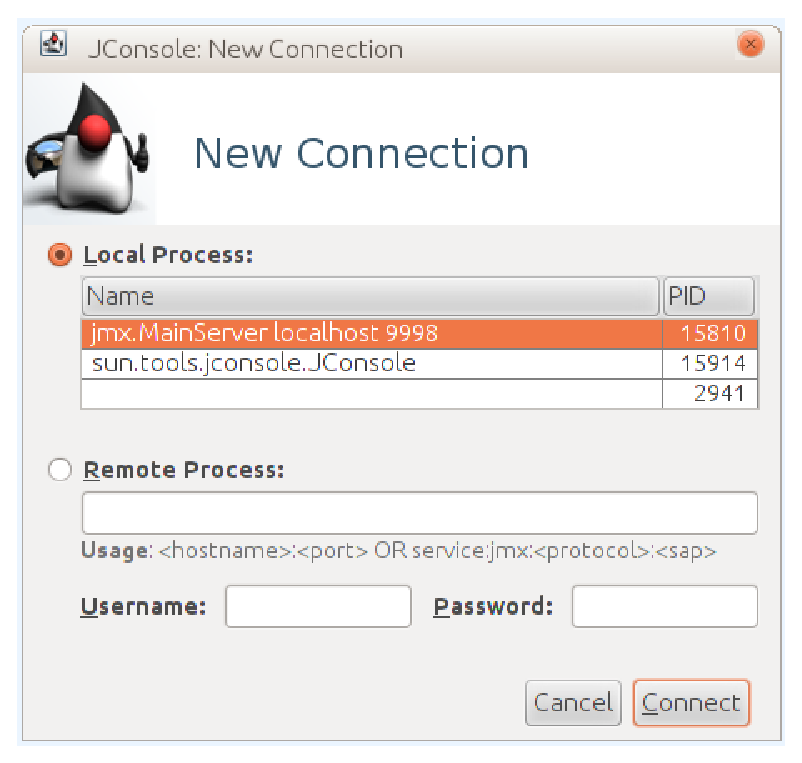
\includegraphics[scale=0.6]{graphics/jConsole.eps}
%\centering
% \caption[JConsole MBeans]{JConsole Angemeldete MBeans}
% \label{fig:JConsole}
%\end{figure}
%
%\begin{figure}[!htb]
%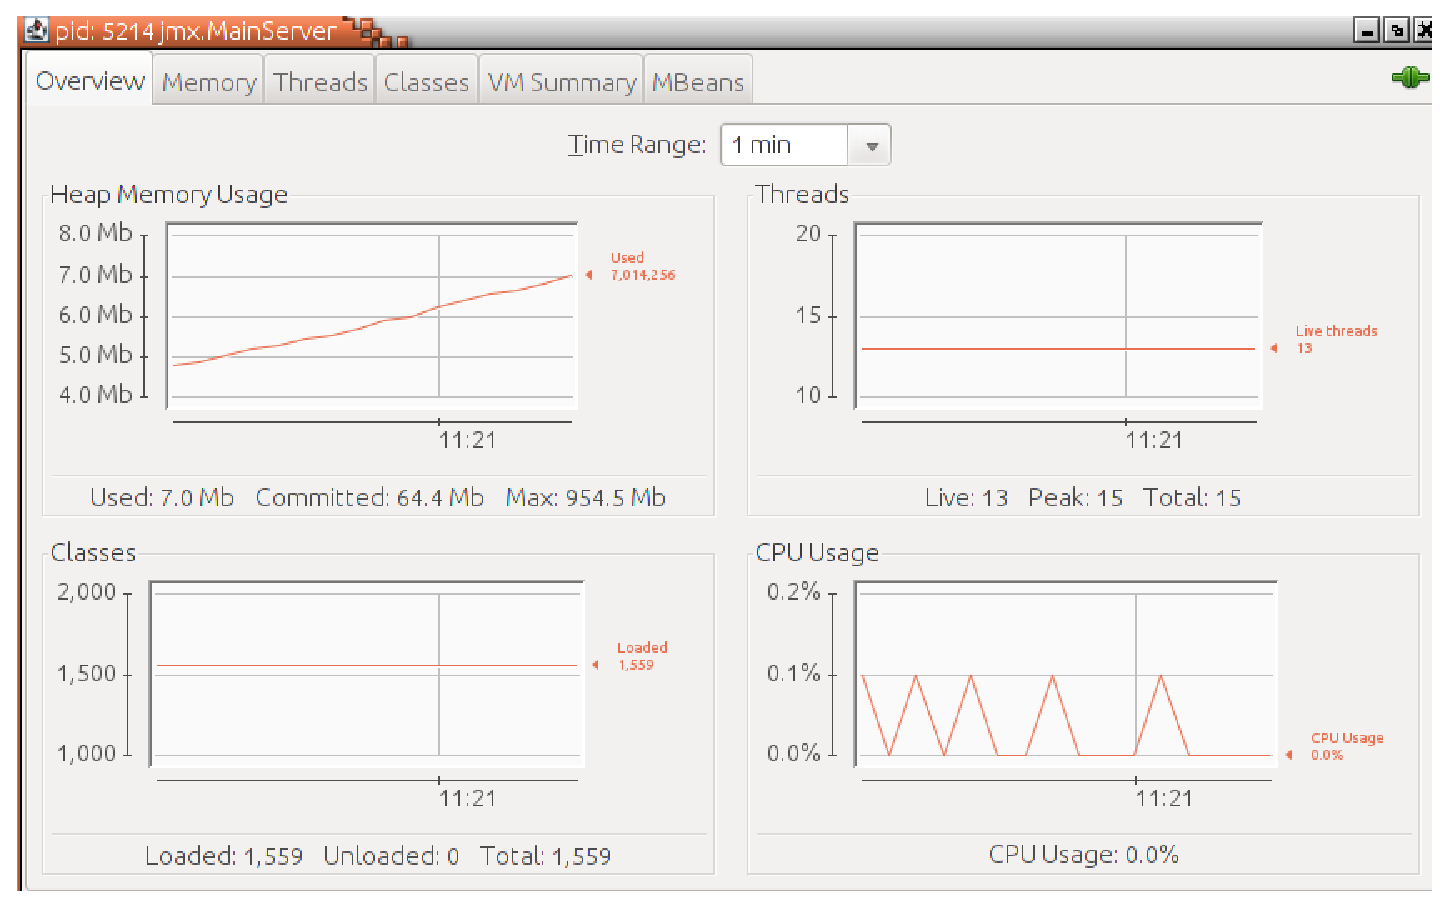
\includegraphics[scale=0.5]{graphics/jConsole2.eps}
%\centering
% \caption[JConsole Monitoring]{JConsole Monitoring}
% \label{fig:JConsole2}
%\end{figure}	
	
	\item Shell-Script: Eine andere Möglichkeit, um beispielsweise einen konsolenbasierten Client zu schrieben, ist durch die Verwendung von jmxterm\footnote{http://wiki.cyclopsgroup.org/jmxterm} gegeben. Daf\"ur ist lediglich ein einfaches Skript f\"ur den Verbindungsaufbau zum MBeanServer und der \"Ubergabe einer Ausf\"uhrungsliste notwendig. Die gew\"unschten Interaktionen werden unter Ber\"ucksichtigung einer gewissen Syntax in diese Liste\footnote{einfache Textdatei} geschrieben und dem Skript als Parameter \"ubergeben. Ein konkretes Beispiel wird im Kapitel Implementierung aufgezeigt.	
	
	\item Webbrowser: F\"ur die Agent-View \"uber einen Webbrowser bietet sich die Nutzung von JMXTools an. Neben dem MBeanServer muss die durch die Library bereitgestellte Klasse \courier{HtmlAdaptorServer} gestartet werden. Dieser wird zusätzlich ein Host und ein Port \"ubergeben. Mittels Webbrowser kann nun über den Host und den Port eine Verbindung zum \courier{MBeanServer} aufgebaut werden. Anschlie\ss end stehen die \courier{MBeans} zur Auswahl bereit. Die Operationen des gewählten \courier{MBeans} lassen sich nun \"uber den Webbrowser steuern.
	
%\begin{figure}[!htb]
%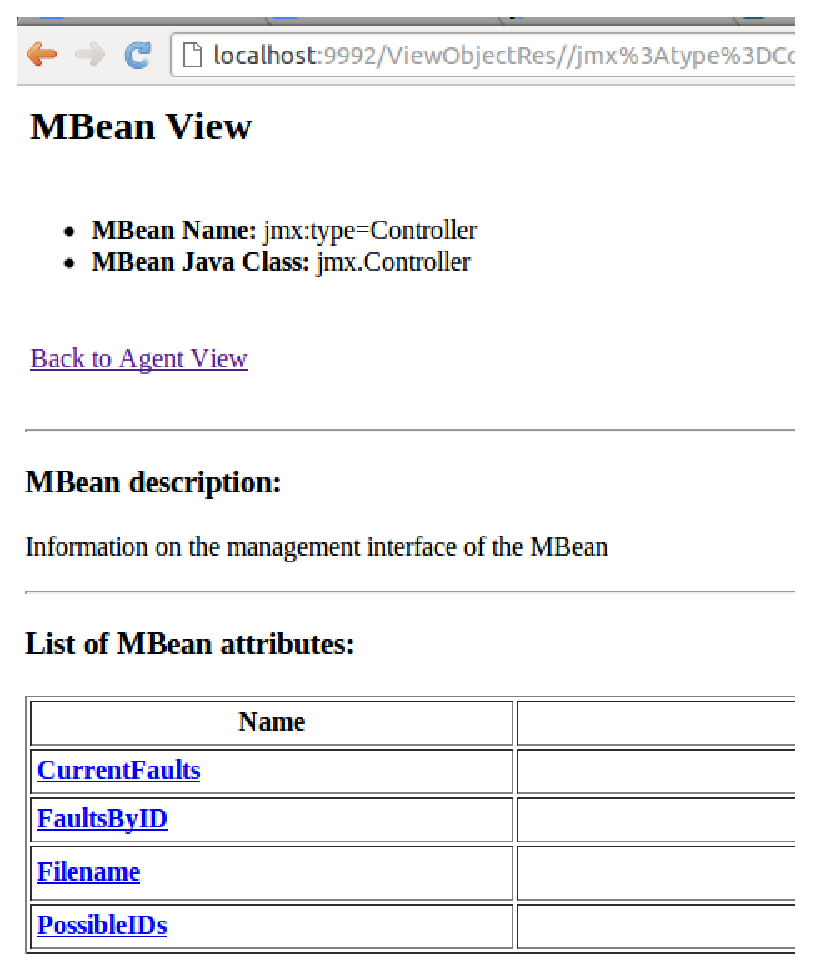
\includegraphics[scale=0.7]{graphics/htmlView.eps}
%\centering
% \caption[HtmlAdaptorServer]{HtmlAdaptorServer}
% \label{fig:HtmlAdaptorServer}
%\end{figure}		
	
	\item Java-Client: Java-Clients lassen sich ebenfalls über die \courier{ControllerMBean} Schnittstelle sehr leicht integrieren. Die Verbindung zum \courier{MBeanServer} wird \"uber RMI oder lokal aufgebaut. Ist die Verbindung erfolgreich können Variablen über \courier{Attribut}-Objekte gesetzt oder erfragt werden. Um die Methoden auszuführen ist ein \courier{Connection}-Objekt erforderlich.
\end{itemize}



%
\section{Sequenzieller Ablauf} 

Den zeitlichen Ablauf der Interaktion zwischen den Hauptklassen zeigt das Sequenzdiagramm aus Abbildung \ref{Sequenzdiagramm}. F\"ur die Nutzung des Programms ist die Anmeldung am MBean-Server als erster Schritt obligatorisch. Dieser stellt die Schnittstelle zum \courier{Controller} bereit, welcher alle erforderlichen Operationen f\"ur den Client verfügbar macht. Im Sequenzdiagramm aus Abbildung \ref{Sequenzdiagramm} ist zur Vereinfachung der Grafik die Verbindung zwischen Client und \courier{Controller} direkt eingezeichnet worden. \\
Nach der erfolgreichen Anmeldung am Server steht es dem Client frei welche Operation er ausf\"uhren m\"ochte. Auf der Zeitlinie aus Abbildung \ref{Sequenzdiagramm} folgt als erster Schritt eine Fehlerwertabfrage, um anhand der ID's neue Werte setzen zu können.\\
Im Anschluss wird die Default Fehlerinjektion vom Client gestartet. Der \courier{Controller} gibt den Aufruf zunächst an den \courier{StreamProcessor} weiter. Der \courier{StreamProcessor} liest die Daten ein und übergibt sie als Byteliste an ein \courier{Context}-Objekt. Die Klasse \courier{Context} wählt anhand der Fehlerwerte, in diesem Fall die Default Fehlerwerte im Quellcode, die erforderliche Strategie aus. Die Bytes werden mit Fehlern injiziert und zurück an den \courier{StreamProcessor} geschickt. 
Der Injektionsaufruf des \courier{Controllers} respektive des Clients wird nun vom \courier{StreamProcessor} durch das Schreiben der Daten in eine vorher angelegte Ausgabedatei zum Abschluss gebracht. \\
Eine Fehlerinjektion mit Streamwechsel ist in Abbildung \ref{Sequenzdiagramm} unter ``RunInjection mit Streamwechsel'' dargestellt. Zuerst wird ein anderer Ausgabestream gewählt. Diese Operation kann zeitlich auch später folgen, muss jedoch vor dem Injektionsaufruf ausgeführt werden. Danach wurden die Fehlerwerte neu gesetzt. Das Setzen der Fehlerwerte kann zu verschiedenen Ausnahmebehandlungen führen. Im Diagramm wurde eine falsche ID übergeben. Der Controller bekommt daraufhin bei der Modifikation der Annotationen eine Fehlermeldung übergeben, welche an den Client weitergereicht wird. Im Falle einer korrekten Übergabe der Fehlerwerte erhält der Controller einen modifizierten \courier{StreamProcessor}. Anschlie\ss end kann die Injektion vom Client veranlasst werden. Der Controller ruft an dieser Stelle die entsprechende Methode des modifizierten \courier{StreamProcessor} auf. Die weitere Verarbeitung geschieht ananlog zur Default Injektion.



\begin{figure}[!htb] 
\centering

\begin{sequencediagram}
\newthread{cl}{:Client}
\newinst[2]{contr}{:Controller}
\newinst[1]{fp}{:StreamProcessor}
\newinst[1]{conte}{:Context}
\newinst{ms}{:MainServer}

\begin{call}
	{cl}	{Anmeldung}{ms}{}
\end{call}

\begin{sdblock}{getCurrentFaults}{}

\begin{call}
	{cl}{gib Fehlerwerte}{contr}{aktuelle Fehlerwerte}
\end{call}

\end{sdblock}

\begin{sdblock}{RunInjection}{}

\begin{call}
	{cl}	{Injektion}{contr}{}
	\begin{call}
		{contr}{Injektion}{fp}{schreibe Daten}
		\begin{call}
			{fp}{übergabe Bytes}{conte}{injiz. Daten}
		\end{call}
	\end{call}
\end{call}

\end{sdblock}


\begin{sdblock}{RunInjection}{mit Streamwechsel}

\begin{messcall}
	{cl}{setze Ausgabestream}{contr}
\end{messcall}

\begin{call}
	{cl}	{setze Fehlerwerte}{contr}{Error ID falsch}
\end{call}

\begin{messcall}
	{cl}	{setze Fehlerwerte}{contr}{}
	\begin{call}
		{contr}{modif. StreamPr.}{fp}{}
	\end{call}
\end{messcall}


\begin{call}
	{cl}	{Injektion}{contr}{}
	\begin{call}
		{contr}{Injektion}{fp}{schreibe Daten}
		\begin{call}
			{fp}{übergabe Bytes}{conte}{injiz. Daten}
		\end{call}
	\end{call}
\end{call}
\end{sdblock}

\end{sequencediagram}

	\caption[Sequenzdiagramm]{Sequenzdiagramm}
 	\label{Sequenzdiagramm}
\end{figure}




%\newpage
%
%\begin{sequencediagram}
%\newthread[red]{r}{:Red}
%\newthread[green]{g}{:Green}
%\newthread[blue]{b}{:Blue}
%\tikzstyle{inststyle}+=[top color=yellow,bottom
%color=gray]
%\newinst{y}{:Yellow}
%\tikzstyle{inststyle}+=[bottom color=white,top
%color=white,rounded corners=3mm]
%\newinst{o}{:Rounded}
%\end{sequencediagram}
%
%\begin{sequencediagram}
%\newthread{ss}{:Client}
%\newinst{ctr}{:Controller}
%\newinst{ps}{:PhysicsServer}
%\newinst[1]{sense}{:FileProcessor}
%\begin{call}{ss}{Initialize()}{sense}{}
%\end{call}
%\begin{sdblock}{RunLoop}{Themainloop}
%\begin{call}{ss}{StartCycle()}{ctr}{}
%\begin{call}{ctr}{ActAgent()}{sense}{}
%\end{call}
%\end{call}
%\begin{call}{ss}{Update()}{ps}{}
%\begin{messcall}{ps}{PrePhysicsUpdate()}{sense}{state}
%\end{messcall}
%\begin{sdblock}{PhysicsLoop}{}
%\begin{callself}{ps}{PhysicsUpdate()}{}
%\end{callself}
%\end{sdblock}
%\begin{call}{ps}{PostPhysicsUpdate()}{sense}{}
%\end{call}
%\end{call}
%\begin{call}{ss}{EndCycle()}{ctr}{}
%\begin{call}{ctr}{SenseAgent()}{sense}{}
%\end{call}
%\end{call}
%\end{sdblock}
%\end{sequencediagram}



\label{Implementierung}
\chapter{Implementierung}\vspace{1cm}
Das folgende Kapitel zeigt die Implementierungsdetails der im Design-Kapitel erläuterten Komponenten. Es werden hierfür die wichtigsten Funktionen beschrieben und zum besseren Verständnis der Code anhand von kurzen Ausschnitten aufgezeigt.\\
Die einzelnen Klassen wurden nach ihrem Aufgabengebiet in verschiedene Java-Pakete eingeteilt. Zunächst wird das Paket \courier{faults} betrachtet. Dessen Inhalte sind alle Klassen die Fehlerwerte repr\"asentieren und daher von den folgenden Klassen verwendet werden.\\
Das Paket \courier{processor} bildet den Hauptteil des Kapites. Es beinhaltet die Klassen  \courier{Context}, \courier{StreamProcessor}, also auch die Klasse \courier{AddRuntimeAnnotation}. Alle drei Klassen sind eng aneinander gekoppelt und für die Hauptfunktionalität der Anwendung zuständig. \\
Die einzelnen Injektions-Logiken wurden in das Paket \courier{strategies} gepackt. In diesem Abschitt steht das verwendete Pattern, welches für die Implementierung der Injektion verwendet wurde, im Fokus. Die vorhandenen Strategien werden nur kurz, anhand einer ausgewählten Strategie exemplarisch vorgestellt.\\
Die Implementierungen des \courier{Controllers} und des \courier{MainServers} sind Bestandteil des Paketes \courier{jmx}. In diesem Abschnitt wird die verwendete JMX-Technologie detailliert beschrieben und anschlie\ss end dessen Verwendung anhand verschiedener JMX-Client Implementierungen aufgezeigt.


\section{Fehlerwerte}
Die Fehlerwerte der zu injizierenden Streams sind im Paket \courier{faults} erstellt worden. Dieses Paket besteht aus einer Klasse, zwei Annotationen und einer Enumeration. In der weiteren Implementierung werden diese Konstrukte an vielen Stellen verwendet und stehen insbesondere bei der dynamischen Anpassung der Fehlerwerte im Fokus.

\begin{enumerate}
	\item FaultInj : Die Annotation \courier{FaultInj} wurde eigens definiert, um die zu injizierenden Streams als fehlerbehaftet kennzeichnen zu können. Sie besteht aus den Werten id, type, rate und blocksize. In Listing \ref{lstFaultInj} ist zu erkennen, dass alle Variablen bis auf die id einen Default-Wert besitzen. Eine Fehlermarkierung kann somit wie in Listing \ref{lstannoStream} vorgenommen werden. In diesem Fall ist zwar eine Markierung vorhanden, es werden aber vorerst keine Fehlerwerte eingestreut. Aufgrund der Eindeutigkeit der ID besitzt sie keinen Default-Wert. Der Entwickler wird somit explizit durch den Compiler zur Angabe einer ID gezwungen. \\
	  
	\lstinputlisting[style=stJava,caption={Annotation FaultInj}, label=lstFaultInj]{listings/FaultInj.java}
	
		  
\lstinputlisting[style=stJava,caption={Annotation Default-Werte}, label=lstannoStream]{listings/annoStream.java}	  
	  
	
	\item FaultInjects : F\"ur Streams, die mehr als einen Fehlerwert erhalten sollen, wurde eine weitere Annotation definiert. Da mehrere Annotationen für eine Variable nicht zulässig sind, wurde dieses Verhalten über einen Umweg erzielt. Die \courier{FaultInject}-Annotation aus Listing \ref{lstFaultInjects} besitzt einen Array vom Typ der urspr\"unglichen \courier{FaultInj}-Annotation. Der Stream wird nun einfach mit der \courier{FaultInject}-Annotation markiert und die gewünschten \courier{FaultInj}-Annotationen dem Array übergeben.\\
	
	\lstinputlisting[style=stJava,caption={Annotation FaultInjects}, label=lstFaultInjects]{listings/FaultInjects.java}
		
	\item FaultType : F\"ur die angebotenen Fehlertypen wurde ein Enum mit dem Namen \courier{FaultType} erstellt (Listing \ref{lstFaultType}). Die Fehlertypen beziehen sich, wie im Design Kapitel erl\"autert, auf die Injektions-Strategie. Soll die Anwendung um eine Fehlerstrategie erweitert werden, kann diese \"uber das Enum \courier{FaultType} dem Client zug\"anglich gemacht werden. Ausschlie\ss lich hier definierte Typen werden von der Anwendung akzeptiert.\\
	
	\lstinputlisting[style=stJava,caption={Enum FaultType}, label=lstFaultType]{listings/FaultType.java}

	\item FaultValue: Die Klasse \courier{FaultValue} dient als Wrapper-Klasse\footnote{Aufname von Daten in ein Objekt} f\"ur die Parameter einer Annotation. Die Klasse erleichtert somit die Datenübergabe an andere Klassen sowie das Auslesen der jeweiligen Fehlerparameter.
\end{enumerate}






%%
\section{Klasse StreamProcessor}
Der \courier{StreamProcessor} ist das Zentrum der Anwendung. Über diese Klasse werden zu Beginn die Daten aus der Datei oder dem Stream gelesen. Die Daten werden anschlie\ss end als einzelne Bytes an die Klasse \courier{Context} übergeben. Dieses Vorgehen ist durch Listing \ref{lstFaultPro2} umgesetzt worden.
\begin{figure}[!htb]
	\lstinputlisting[style=stJava,caption={StreamProcessor Einlesen der Daten}, label=lstFaultPro2]{listings/FileProcessor2.java}
\end{figure}
F\"ur das Einlesen der Daten wurde ein \courier{InputStream} verwendet. Dieser Stream wird von \courier{FileIO}, \courier{Sockets}, etc. unterstützt. Der fehlerbehaftete Stream muss global deklariert sein, damit er annotiert/injiziert werden kann. Die beiden M\"oglichkeiten der Annotierung sind durch Listing \ref{lstFaultPro1} gegeben.\\
Im n\"achsten Schritt wird der \courier{InputStream} durch die Methode \courier{readStream} in eine Byte-Liste ausgelesen. Aufgerufen wurde \courier{readStream} durch die Methode \courier{loadStream}, welche die erstellte Ergebnisliste bzw. den Datensatz mit einer dazugehörigen ID an das \courier{Context} Objekt übergibt. Im zweiten Schritt werden die Fehlerwerte durch die Methode \courier{setFaultsByIDToContext} unter Verwendung von Java Reflection \footnote{http://docs.oracle.com/javase/tutorial/reflect/index.html - Zugriff am 21. Juli 2012
} an das \courier{Contex} Objekt übergeben. Die Methode benötigt dafür die Fehler-ID's und die ID des betroffenen Datensatzes.
\begin{figure}[!htb]
	\lstinputlisting[style=stJava,caption={StreamProcessor Fehlermarkierung}, label=lstFaultPro1]{listings/FileProcessor1.java}
\end{figure}
Das Laden der Daten wird beim Aufruf der Methode \courier{processData} aus Listing \ref{lstFaultPro3} veranlasst. Nach dem Laden folgt die Methode \courier{injectFaults} der Klasse \courier{Context}. Diese sorgt intern daf\"ur, dass die verwalteten Daten mit den beigef\"ugten Fehlerwerten injiziert werden.\\
F\"ur das Auslesen der manipulierten Daten aus dem \courier{Context} Objekt, sowie das Schreiben in eine neue Datei wurde die innere Klasse \courier{Reducer} implementiert. Der \courier{Reducer} erstellt zun\"achst den Stream für die Ausgabe und bereitet eine neue Datei vor. Danach wird die Methode \courier{reduce} aufgerufen um durch den jeweiligen Datensatz zu iterieren und die Bytes durch den gewählten Stream in die neue Datei zu schreiben.
\begin{figure}[!htb]
	\lstinputlisting[style=stJava,caption={StreamProcessor Einlesen/Injektion/Ausgabe}, label=lstFaultPro3]{listings/FileProcessor3.java}
\end{figure}
Das Auslesen der \courier{FaultValues} ist durch die Implementierung aus Listing \ref{lstFaultPro4} realisiert worden. Diese Methode wird ebenfalls im \courier{Controller/MBeanController} verwendet, um  auf Anfrage des Clients die Fehlerwerte liefern. Die Funktion arbeitet mit der bereits erw\"ahnten Java Reflection Technologie um die injizierten Felder zu ermitteln. Es werden alle globalen Variablen durchgegangen und \"uberpr\"uft, ob die \courier{FaultInjects} Annotation präsent ist. Ist dies der Fall, werden alle \courier{FaultInj} Annotationen heraus gefiltert und deren Fehlerwerte als \courier{FaultValue} verpackt zu einer Liste beigef\"ugt. F\"ur den Fall, dass statt einer \courier{FaultInjects} Annotation nur eine einzelne \courier{FaultInj} Annotation vorhanden ist, wird im \courier{else}-Zweig die Verarbeitung analog f\"ur die einzelne \courier{FaultInj} durchgef\"uhrt.
\begin{figure}[!htb]
	\lstinputlisting[style=stJava,caption={StreamProcessor Fehlerwertrückgabe}, label=lstFaultPro4]{listings/FileProcessor4.java}
\end{figure}
%%
\section{Klasse AddRuntimeAnnotation}

Für die dynamische Konfiguration der Fehlerwerte wurde die Klasse \courier{AddRuntimeAnnotation} geschrieben. Sie enthält eine statische Methode \courier{addFaultInjAnnotationToMethod} die für die Umsetztung der Modifikation zuständig ist. Bei ihrer Ausführung ver\"andert sie die Class Datei des StreamProcessors und liefert als Resultat eine Instanz des modifizierten Objektes zurück. Die Methode wurde so konzipiert, dass mehrere Annotationen mit einem Aufruf ge\"andert werden k\"onnen. F\"ur die Modifikation nutzt die Methode verschiedene Komponenten aus der Library javassist.\\
Eine in der Implementierung aus Listing \ref{lstAddRun1} benutzte Komponente ist die Klasse \courier{Javassist.CtClass}\footnote{compile-time class}, welche die Class Datei des StreamProcessors repr\"asentiert. Um eine solche \courier{CtClass} erstellen und sp\"ater modifizieren zu k\"onnen wurde vorher ein \courier{ClassPool} Objekt erstellt. Der \courier{ClassPool} liest mittels des Schl\"usselworts \courier{get} die gew\"unschte Class Datei und konstruiert aus dieser eine \courier{CtClass}. Die \courier{CtClass} kann nun auf Bytecode-Ebene angepasst werden. Um den Bytecode des StreamProcessors updaten zu können, wurde ein Objekt vom Typ \courier{HotSwapper} erstellt. Dieses ben\"otigt lediglich einen Port für das Laden der neuen Class Datei\footnote{inter-thread communication}. Die Umsetzung der Erstellung dieser Komponenten wird in Listing \ref{lstAddRun1} gezeigt.

\begin{figure}[!htb]
	\lstinputlisting[style=stJava,caption={Initialisierung HotSwapper \& CtClass}, label=lstAddRun1]{listings/AddRuntime1.java}
\end{figure}

Als Parameter bekommt die Methode \courier{addFaultInjAnnotationToMethod} die neuen Fehlerwerte anhand eines \courier{FaultValue} Array \"ubergeben. Mittels der ID des jeweiligen FaultValues kann, wie in Listing \ref{lstAddRun2} zu sehen, das dazugeh\"orige Feld in der Klasse \courier{StreamProcessor} bestimmt werden. Die ermittelten Felder bekommen f\"ur den Manipulationsvorgang eine Instanz der Klasse \courier{Javassist.CtField} zugewiesen. 

\begin{figure}[!htb]
	\lstinputlisting[style=stJava,caption={Bestimmung injizierter Felder}, label=lstAddRun2]{listings/AddRuntime2.java}
\end{figure}

Um neue Felder, Methoden, Annotationen etc. hinzuf\"ugen zu k\"onnen wurde ein \courier{ClassFile} Objekt auf den \courier{CtClass} Class-File referenziert. Zus\"atzlich wurde ein \courier{ConstPool}\footnote{constant pool table} Objekt mit Verweis auf diesen Class-File erstellt (Listing \ref{lstAddRun3}). 
Für die neuen Annotationen wurden zwei \courier{javassist.Annotation} Objekte definiert. Eines f\"ur die \courier{FaultInjects} und das andere Objekt f\"ur die \courier{FaultInj} Annotationen. Ein \courier{AnnotationsAttribute} Objekt ist nach der Erstellung der Annotationen f\"ur die \"Ubergabe an das entsprechende \courier{ctField} notwendig. 

\begin{figure}[!htb]
	\lstinputlisting[style=stJava,caption={Neue Annotationen}, label=lstAddRun3]{listings/AddRuntime3.java}
\end{figure}

F\"ur die Erstellung der neuen Annotationen wurde zun\"achst durch die vorher bestimmten \courier{CtFelder} iteriert. Es wurde die alte Annotation bestimmt und eine neue Annotation dieses Typs (\courier{FaultInjects} oder \courier{FaultInj}) angelegt (Listing \ref{lstAddRun4}). Die erstellten Annotationen wurden gleichzeitig zur Speicherung, der constant-pool-table beigef\"ugt. 

\begin{figure}[!htb]
	\lstinputlisting[style=stJava,caption={Zuweisung des Annotationstyps}, label=lstAddRun4]{listings/AddRuntime4.java}
\end{figure}

Im \courier{if}-Zweig, also falls ein Feld mit einer \courier{FaultInjects}-Annotation pr\"asent ist, wird ein \courier{AnnotationMemberValue} Array f\"ur die Unterannotationen verwendet. Es werden zun\"achst alle Unterannotationen durchlaufen und nach der passenden ID gesucht. Falls die ID gefunden wurde, können die neuen Fehlerwerte aus dem \courier{FaultValue} Array geschrieben werden. F\"ur alle anderen Unterannotationen wurden die alten Werte erneut verwendet. Nach jedem Durchlauf wird die erstellte Unterannotation dem \courier{AnnotationMemberValue} Array \"ubergeben. Dieser repr\"asentiert die \courier{FaultInjects}-Annotation und kann im Anschluss komplett an das \courier{Annotation} Array übergeben werden (Listing \ref{lstAddRun5}).  \\
Im \courier{else}-Zweig, falls also ein Feld mit einer \courier{FaultInj}-Annotation pr\"asent ist, werden lediglich die neuen Werte in die Annotation aufgenommen. Da im anfangs erstellten \courier{CtField} Array nur Felder enthalten sein k\"onnen die ge\"andert werden sollen, muss hier auch keine weitere \"Uberpr\"ufung durchgef\"uhrt werden.\\
Zum Schluss kommt das \courier{AnnotationsAttribute} Objekt zum Einsatz. Jede Annotation wird diesem Objekt \"ubergeben und die Sichtbarkeit zur Laufzeit gesetzt. Dann kann dieses dem entsprechenden \courier{CtField} \"ubergeben werden.

\begin{figure}[!htb]
	\lstinputlisting[style=stJava,caption={Setzen der Fehlerwerte}, label=lstAddRun5]{listings/AddRuntime5.java}
\end{figure}

Nachdem die Klasse mit den neuen Annotationen versehen wurde, muss der Bytecode neu geladen werden. Hierf\"ur  wird das \courier{CtClass} Objekt in eine Class Datei transformiert und anschlie\ss end der Bytecode ausgelesen. Die Klasse \courier{javassist.HotSwapper} l\"adt nun anstelle des urspr\"unglichen, den modifizierten Bytecode erneut in die JVM (Listing \ref{lstAddRun6}).

\begin{figure}[!htb]
	\lstinputlisting[style=stJava,caption={Laden des Bytecodes}, label=lstAddRun6]{listings/AddRuntime6.java}
\end{figure}

%constant pool table, an array of variable-sized constant pool entries, containing items such as literal numbers, strings, and references to classes or methods. Indexed starting at 1, containing (constant pool count - 1) number of entries in total (see note).
%
%The constant pool table is where most of the literal constant values are stored. This includes values such as numbers of all sorts, strings, identifier names, references to classes and methods, and type descriptors. All indexes, or references, to specific constants in the constant pool table are given by 16-bit (type u2) numbers, where index value 1 refers to the first constant in the table (index value 0 is invalid).







%
\section{Context}

Die Klasse \courier{Context} ist f\"ur die Datenverwaltung/-manipulation verantwortlich. In Listing \ref{lstContext1} ist die Methode \courier{write} zu sehen die vom \courier{StreamProcessor} zur \"Ubergabe der Datens\"atze aufgerufen wird. Als Prämisse dafür gilt die Serialisierbarkeit der Daten. Zur Erfassung wurde eine \courier{HashMap} gewählt, über die eine einfache Verwaltung der Datensätze anhand der ID möglich ist.

\begin{figure}[!htb]
	\lstinputlisting[style=stJava,caption={Context: Einlesen der Datensätze}, label=lstContext1]{listings/Context1.java}
\end{figure}

Um die Daten mit Fehlern zu injizieren, wurde die Methode \courier{getStrategy} aus Listing \ref{lstContext2} erstellt. Die Methode bekommt einen Datensatz mit dem dazugehörigen Fehlerwert als Parameter \"ubergeben. Anhand des Fehlertyps wird die zugrundeliegende Strategie ausgewählt. 
Neue Strategien müssen in diese Methode integriert werden.

\begin{figure}[!htb]
	\lstinputlisting[style=stJava,caption={Context: Strategieauswahl}, label=lstContext2]{listings/Context2.java}
\end{figure}

Die gew\"ahlte Strategie kann nun in der Methode \courier{injectFaults} f\"ur die Dateninjektion verwendet werden (Listing \ref{lstContext3}). Die Variable \courier{registeredFaultInjectors} ist eine Liste, bestehend aus Tupeln von IDs\footnote{Referenz auf Datensätze} und dazugeh\"origen \courier{FaultValues}. Im Gegensatz zu den Datens\"atzen der \courier{HashMap} sind bei dieser Liste die IDs nicht eindeutig, da jeder Datensatz mehrere \courier{FaultValues} haben kann. Die gew\"ahlte Strategie bekommt diese Werte \"ubergeben und ruft ihrerseits die Methode \courier{runInjection} auf. 

\begin{figure}[!htb]
	\lstinputlisting[style=stJava,caption={Context: Injektionsausführung}, label=lstContext3]{listings/Context3.java}
\end{figure}
%
\section{Fehler Injektion}

Die Implementierung der Fehlerinjektionen wurde mittels einer abgewandelten Form des Strategy Patterns realisiert. Die abstrakte Klasse \courier{InjectionStrategy} dient als Oberklasse aller  konkreten Strategien. Sie stellt für ihre Unterklassen die beiden Funktionen aus Listing \ref{lstFaultInjector1} bereit. Die Methode \courier{isInjected} ist f\"ur jede Strategie gleich und wird daher bereits mit Funktionalit\"at an die Unterklassen vererbt. \courier{isInjected} ist f\"ur den Funken Zufall in den einzelnen Injektionen verantwortlich. Anhand der Fehlerrate, die zwischen 0 und 1 liegen muss und einem Zufallswert der ebenfalls zwischen 0 und $<$1 liegt, wird entschieden ob ein Bit bzw. Block injiziert werden soll.\\
Die zweite Methode ist mit dem Schl\"usselwort \courier{abstract} deklariert. Die Implementierung der eigentlichen Algorithmen finden sich erst in der Methode \courier{runInjection} der jeweiligen Unterklassen wieder.\\
Verwendet wird dieses Muster in der bereits beschriebenen Klasse \courier{Context} durch die Methode \courier{getInjectionStrategy}. Diese Methode erzeugt eine Member-Variable aus der abstrakten Klasse \courier{InjectionStrategy}, die mit einer Referenz auf die gew\"unschte Logik belegt ist. Somit kann eine konkrete Strategie beliebig eingebunden als auch ausgetauscht werden. Die Implementierung ist dadurch sehr leicht erweiterbar. Insgesamt benötigen neue Strategien folgende Anpassungen/Erweiterungen:

\begin{itemize}
		\item einen eigenen Typ im \courier{Enum FaultType}
		\item müssen von der aktrakten Klasse \courier{InjectionStrategy} erben und dessen abstrakte Methode \courier{runInjection} implementieren.
		\item müssen in die Methode \courier{getStrategy} der Klasse \courier{Context} integriert werden
	\end{itemize}
	
\begin{figure}[!htb]
	\lstinputlisting[style=stJava,caption={InjectionStrategy}, label=lstFaultInjector1]{listings/FaultInjector1.java}
\end{figure}



\section{JMX Implementierung}

\subsection{Controller/MainServer}

Als Schnittstelle zwischen Benutzer und Anwendung wurde die Klasse \courier{Controller} eingef\"uhrt. Sie wird vom Anwender \"uber den sogenannten MBean-Server angesprochen. Die Klasse \courier{Controller} ist in der Anwendung f\"ur die Steuerung der Fehlerinjektion und weiteren Funktionalitäten verantwortlich. Der Client bekommt die f\"ur ihn vorgesehene Funktionalit\"at durch das Interface \courier{ControllerMBean} aus Listing \ref{lstController2}. Das Interface stellt alle nach au\ss en sichtbaren Methoden bereit und muss vom \courier{Controller} implementiert werden. Der \courier{Controller} ist somit \"uber das Interface ansprechbar, alle weiteren Implementierungsdetails bleiben nach au\ss en verborgen.

\begin{figure}[!htb]
	\lstinputlisting[style=stJava,caption={ControllerMBean}, label=lstController2]{listings/Controller2.java}
\end{figure}

Die Implementierung des \courier{MainServer} ist in Listing \ref{lstController3} dargestellt. Um die Java Management Extensions nutzen zu k\"onnen, muss zun\"achst ein \courier{MBeanServer} Objekt durch den Aufruf der Methode \courier{getPlatformMBeanServer} der Klasse \courier{java.lang.management.ManagementFactory} erstellt werden. Danach wird ein \courier{ObjectName} f\"ur das zu erstellende \courier{Controller} MBean definiert. Dieses besteht aus einer Domain und einer Liste von key-properties. Die Domain ist das \courier{package} in dem sich das zu erstellende MBean befindet. In Listing \ref{lstController3} ist dies das \courier{package jmx}. Die key-property spezifiziert den Typen des Objektes, in diesem Fall der Typ \courier{Controller}. Im Anschluss wird eine Objektinstanz des \courier{Controllers} erzeugt. Dieses kann nun als MBean mit dem \courier{ObjectName} Objekt am \courier{MBeanServer} registriert werden. Nach dem Starten der Klasse \courier{MainServer} wird auf die Aufrufe der im \courier{ControllerMBean} definierten Methoden gewartet, welche dann \"uber den \courier{Controller} ausgef\"uhrt werden.

\begin{figure}[!htb]
	\lstinputlisting[style=stJava,caption={MainServer}, label=lstController3]{listings/Controller3.java}
\end{figure}

 F\"ur die M\"oglichkeit einer zus\"atzlichen RMI Connection wurde die Implementierung aus Listing \ref{lstController1} verwendet. Falls keine Parameter mitgegeben wurden, wird die Klasse \courier{Mainserver} wie bisher gestartet. Andernfalls existiert die Klasse \courier{JMXServiceURL} aus \courier{javax.manage-\\ment.remote}, der sich Hostname und Port als Parameter \"ubergeben lassen. Die somit erstellte URL wird mit dem MBean Server \"uber einen \courier{JMXConnectorServer} verkn\"upft.

\begin{figure}[!htb]
	\lstinputlisting[style=stJava,caption={MainServer RMI}, label=lstController1]{listings/Controller1.java}
\end{figure}

\subsection{Client Implementierung}

JMX-Clients gibt es bereits in vielen Variationen. Sehr beliebt sind die JConsole, Java-, Shell- oder HTML-Clients\footnote{http://www.servletsuite.com/jmx/jmx-html.htm - Zugriff am 09. September 2012}. Im Folgenden werden ein Shell-Skript und eine Java Client Implementierung vorgestellt.

\subsubsection{Shell-Skript}
 F\"ur das Bash-Script wurde die jmxterm-1.0 library verwendet. Diese bietet eine intuitive Handhabung und ermöglicht einen einfachen Verbindungsaufbau. Der implementierte Client besteht aus einer bash-Datei f\"ur den Verbindungsaufbau und dem Starten der jmxterm.jar mit einer Ausf\"uhrungsliste. F\"ur eine RMI-Connection gen\"ugt der Aufruf der jmxterm library mit der entsprechenden Service URL. Die lokale Verbindung aus Listing \ref{lstscript} muss zun\"achst den erforderlichen \courier{MainServer} Process\footnote{jps: Java Virtual Machine Process Status Tool} bestimmen und diesen anschlie\ss end mit dem Schl\"usselwort open der Ausf\"uhrungsliste beif\"ugen. Der open Befehl \"offnet entweder eine neue JMX-Session oder gibt die aktuelle Verbindung wieder.
Eine Ausf\"uhrungsliste ist eine zus\"atzliche Text-Datei, die Anweisungen f\"ur den direkten Verbindungsaufbau zum \courier{MainServer} und alle gew\"unschten Methodenaufrufe erfasst.  

\begin{figure}[!htb]
	\lstinputlisting[style=stBash,nolol=true]{listings/run.sh}
	\lstinputlisting[caption={Bash-File und Ausf\"uhrungsliste}, captionpos=b, label=lstscript]{listings/script.txt}
\end{figure}

\subsubsection{Java Client}

Die Erstellung eines Java Clients verl\"auft relativ analog wie das eben beschriebene Beispiel. Zun\"achst wird wieder die JMX Verbindung per RMI oder Lokal aufgebaut. Danach wird ein \courier{MBeanServerConnection} Objekt erstellt \"uber dessen alle Methodenaufrufe ausgef\"uhrt werden. Sollen beispielsweise ein \courier{FaultValue} gesetzt werden, wird die Methode \courier{setFaultValue} in ein \courier{Attribute} Objekt verpackt und anschlie\ss end der \courier{MBeanServerConnection} mittels dessen Methode \courier{setAttribute} \"ubergeben. Getter-Methoden wie \courier{getCurrentFaults} k\"onnen analog mit \courier{getAttribute} ausgewertet werden. Handelt es sich bei einer Methode nicht um ein \courier{Attribute}\footnote{getter-/setter-Methoden mit nur einem Parameter} wird die Methode \courier{invoke} der \courier{MBeanServerConnection} verwendet. Diese bekommt als Parameter das \courier{ObjectName} Objekt, den Methodennamen und dessen Parameterwerte, als auch die Methodensignatur.

\newpage
\phantom{dd}
\begin{figure}[t!]
	\lstinputlisting[style=stJava,caption={Java Client}, captionpos=b, label=lstclient]{listings/Client1.java}
\end{figure}

%\subsubsection{HTML Adapter}
%
%Eine Connection \"uber einem HTML Adapter wird wie in Listing \ref{lsthtml} implementiert. Das Muster ist wieder dem der vorangegangen Clients sehr \"ahnliche. Zun\"achst wird eine Server-Connection aufgebaut und die Domain des Controller gew\"ahlt. Anschlie\ss end kann der HtmlAdaptorServer und das ObjectName Objekt sich am MBeanServer registrieren. Durch den Aufruf von http://localhost:9992 im Webbrowser kann \"uber den Adapter aus Listing \ref{lsthtml}, auf das Controller MBean zugegriffen werden.
%
%\begin{figure}[!htb]
%	\lstinputlisting[style=stJava,caption={Java Client}, captionpos=b, label=lsthtml]{listings/html.java}
%\end{figure}



%
%
%
%
%
%

\chapter{Evaluation/Messungen}\vspace{1cm}
\label{chp:eval}
% colors
\definecolor{turquoise}{rgb}{0 0.41 0.41}
\definecolor{rouge}{rgb}{0.79 0.0 0.1}
\definecolor{vert}{rgb}{0.15 0.4 0.1}
\definecolor{mauve}{rgb}{0.6 0.4 0.8}
\definecolor{violet}{rgb}{0.58 0. 0.41}
\definecolor{orange}{rgb}{0.8 0.4 0.2}
\definecolor{bleu}{rgb}{0.39, 0.58, 0.93}



Im Kapitel Evalution/Messungen soll das in dieser Arbeit implementierte Programm analysiert und bewertet werden. Gemessen wurden das Einlesen und Schreiben der Daten, die dynamische Konfiguration der Fehlerwerte, sowie der Injektionsvorgang mit den verschiedenen Injektionsstrategien. Im Fokus der Messungen stand prim\"ar die Laufzeit der Fehlerinjektionen, ebenso wurden CPU-Auslastung und Speicherverbrauch untersucht. 

\section{Testaufbau} 
F\"ur die Messungen der Funktionen wurde der folgende Testaufbau umgesetzt: Softwareseitig wurde das System Ubuntu 12.04 mit der Kernel Version 3.2.0-26-generic-pae eingesetzt. Die verwendete Javassist Library ist in Version 3.12.0.GA in die Anwendung integriert worden. Auf der Hardwareseite wurde ein Intel Core i7-2630QM Prozessor mit 8 $\times$ 2.00GHz und einem Arbeitsspeicher von 7.8 GiB verwendet.\\
Die konkreten Messergebisse konnten mit Hilfe des Tools VisualVM Version 1.3.4\footnote{http://visualvm.java.net/relnotes.html - Zugriff 16.09.12} bestimmt werden. Das Tool zeichnet die Aktivit\"aten eines gew\"ahlten Prozesses auf und gibt diese als Diagramm im Reiter Monitor wieder. Alle Laufzeitmessungen wurden direkt im Java Code integriert. Als Testinput dient eine 51.2MB gro\ss e, durch den Output von /dev/zero\footnote{Unix virtuelle Gerätedatei, liefert Null-Bytes}, generierte Datei. Die getesteten Methoden wurden nicht separat sondern, wie in der Anwendung auch, \"uber das \courier{Controller}-Objekt aufgerufen. Die Messung der Strategien wurden jeweils f\"ur die Blockgr\"o\ss en 1, 8, 128, 1024 und 2048 mit den Fehlerraten 1\%, 5\%, 10\%, 50\% und 100\% durchgef\"uhrt.

\section{Lese- und Schreiboperatinen}

F\"ur die Analyse der Einleseoperation ist die Method \courier{loadStream} evaluiert worden. Die folgenden Messwerte aus Tabelle \ref{tblEinlesen} beziehen sich auf das Einlesen der 51.2 MB Datei und der Daten\"ubergabe an das \courier{Context} Objekt.\\
Die Laufzeitmessungen der Methode \courier{loadStream} ergaben einen Mittelwert von 2650 Millisekunden. Versuche mit anderen Java Streams konnten keine nennenswerten Verbesserungen erzielen. Die CPU-Auslastung der Methode stieg bei den Messungen durchschnittlich auf 20\% bis 25\% an. Der Speicherverbrauch lag bei den knapp unter 600 MB. Beim Schreiben der Daten durch die beiden unterschiedlichen Streams war der Laufzeitunterschied signifikanter. Die \courier{reduce} Methode wurde mit dem \courier{ObjectOutputStream} f\"ur serialisierbare Objekte und dem \courier{FileChannel} getestet. Die Umsetzung mit dem \courier{FileChannel} hat eine durchschnittliche Laufzeit von ca. 242 ms. Zum Schreiben der Daten als persistentes Objekt in Form der kompletten Java Liste bedarf es hingegen 113,88 Sekunden.\\

\begin{table}[!htbp]
\centering
\begin{tabular}{c|c|c|c|}
loadStream & Laufzeit & CPU-Last & Speicher\\
\hline
& 2650 ms & 20\% bis 25\% & $<$600 MB\\
\end{tabular}
\caption{Messwerte Einlesen und Daten\"ubergabe}
\label{tblEinlesen}
\end{table}

\section{Dynamische Konfiguration der Fehlerwerte}

Der folgende Test bezieht sich ausschlie\ss lich auf die Funktionalit\"at der dynamischen Fehlerregulierung bzw. der Manipulierung der Annotationen zur Laufzeit. F\"ur die Messungen wurden einem aktiven Stream der Klasse \courier{StreamProcessor} 50 \courier{FaultInj} Annotationen beigef\"ugt. Im Testlauf wurden alle 50 Annotationen mit neuen Werten belegt und die Klasse \courier{StreamProcessor} neu geladen.\\
Die Laufzeitmessung ergab einen Durschnittswert von 1.01 Sekunden. F\"ur den Normalfall einer einzelnen Fehlermodifikation liegt der Wert bei 220 ms. Demnach wird die meiste Zeit f\"ur den Reload des modifizierten \courier{StreamProcessor's} verwendet. Die CPU-Auslastung und der Speicherverbrauch sind in Abbildung \ref{tblDymFehler} grafisch dargestellt. Bei der CPU-Auslastung konnte ein kontinuierlicher Anstieg bis auf knapp 20\% ermittelt werden. Der Speicherverbrauch stieg w\"ahrend der Methodenausf\"uhrung von 10 auf 15 MB nur geringf\"ugig an. 

\begin{figure}[!htb]

\begin{minipage}{7.5cm}

%1950=0 4
\psset{xunit=0.1cm, yunit=0.1cm } 
\begin{pspicture}(-15 , -20)(50,60)
\psaxes[Dx=1, dx=50, Dy=10, dy=10, Ox=0]{->}(60,60) % x=70*0.1=7cm; Dx shown start value; dx*0.1 is distance 
\uput[-90](30,-8){\textcolor{blue}{Zeit in s}}
\uput[180]{90}(-10,30){\textcolor{blue}{CPU-Last in \%}}
\readdata{\data}{cpuAnno.dat} 
\listplot[showpoints=true,linecolor=red, linewidth=1.5pt]{\data}
\end{pspicture}

\end{minipage}
\begin{minipage}{7cm}

%1950=0 4
\psset{xunit=0.1cm, yunit=0.1cm } 
\begin{pspicture}(-20 ,-20)(50,60)
\psaxes[Dx=1, dx=50, Dy=10, dy=10, Ox=0]{->}(60,60) % x=70*0.1=7cm; Dx shown start value; dx*0.1 is distance 
\uput[-90](30,-8){\textcolor{blue}{Zeit in s}}
\uput[180]{90}(-10,30){\textcolor{blue}{Speicherverbrauch in MB}}
\readdata{\data}{memoryAnno.dat} 
\listplot[showpoints=true,linecolor=red, linewidth=1.5pt]{\data}
\end{pspicture}

\end{minipage}

\caption{Messung dynamische Fehlerregulierung}
\label{tblDymFehler}
\end{figure}


\section{Injektionsstategien}

\definecolor{myblue}{HTML}{92dcec}
\newcommand\VRule[1][\arrayrulewidth]{\vrule width #1}

\subsection*{Strategie Random}

Die Random Strategie hat von allen Block-Strategien die l\"angste Laufzeit. Dies resultiert aus der zus\"atzlichen Generierung von zuf\"alligen Bytes.\\
In Abbildung \ref{diaRandom} ist zu sehen wie die Laufzeit bei einer Blockvergr\"o\ss erung sehr stark abnimmt, im Vergleich zu den \"ubrigen Strategien. Je gr\"o\ss er der Block, um so seltener muss die Zufallsgenerierung aufgerufen werden. Sie kann in diesem Fall bereits die Bytes für den ganzen Block in einer Interation generieren. Bei einer Blockgr\"o\ss e von 1 ruft die Funktion f\"ur jedes zu injizierende Byte die Zufallsgenereriung erneut auf, was zu einem Anstieg der Laufzeit f\"uhrt. \\
Entsprechend verh\"alt es sich auch mit der Fehlerrate, wie die Werte aus Tabelle \ref{tblRandom} verdeutlichen. Bei einer steigenden Fehlerrate verl\"angert sich die Laufzeit, da mehr Bytes injiziert werden m\"ussen und entsprechend häufig eine Zufallsgenerierung verlangt wird. Dementsprechend m\"ussen bei einer Fehlerrate von 1.0 f\"ur jeden Block neue Zufallsbytes erstellt werden, was zu einem deutlichen Mehraufwand f\"uhrt. \\ 

\begin{table}[!htb]

\begin{tabular}{rrrrrrr}
\hline\\
\multicolumn{0}{c}{\colorbox{myblue}{\textbf{RANDOM}}} &  
\multicolumn{0}{c}{\colorbox{myblue}{\textbf{Block}}} &  
\multicolumn{0}{c}{\colorbox{myblue}{\textbf{Rate: 0.01}}} &  
\multicolumn{0}{c}{\colorbox{myblue}{\textbf{Rate: 0.05}}} & 
\multicolumn{0}{c}{\colorbox{myblue}{\textbf{Rate: 0.1}}} &
\multicolumn{0}{c}{\colorbox{myblue}{\textbf{Rate: 0.5}}} & 
\multicolumn{0}{c}{\colorbox{myblue}{\textbf{Rate: 1.0}}}\\
 & 1 & 2.84 s & 2.91 s & 3.00 s & 3.85 s & 4.37 s \\
 & 8 & 0.85 s & 0.86 s & 0.89 s & 1.33 s & 1.69 s \\
 & 128 & 0.58 s & 0.59 s & 0.65 s & 0.96 s & 1.30 s \\ 
 & 1024 & 0.54 s & 0.58 s & 0.62 s & 0.91 s & 1.28 s \\
 & 2048 & 0.53 s & 0.57 s & 0.61 s & 0.90 s & 1.26 s \\
\hline
\end{tabular}
\caption{Messwerte Random Strategie}
\label{tblRandom}
\end{table}
\begin{figure}[!htb]

\begin{tikzpicture}
	
	\drawlegend		
 
  \draw (0cm,0cm) -- (13.5cm,0cm);  %Abzisse
  \draw (0cm,0cm) -- (0cm,-0.1cm);  %linkes Ende der Abzisse
  \draw (13.5cm,0cm) -- (13.5cm,-0.1cm) node [right] {Rate}; %rechtes Ende der Abzisse
  
  \draw (-0.1cm,0cm) -- (-0.1cm,5.5cm);  %Ordinate
  \draw (-0.1cm,0cm) -- (-0.2cm,0cm);  %unteres Ende der Ordinate
  \draw (-0.1cm,5.5cm) -- (-0.2cm,5.5cm) node [left] {t in s};  %oberes Ende der Ordinate

  \foreach \x in {2,4,6,8,10}  %Hilfslinien
    \draw[gray!50, text=black] (-0.2 cm,0.5*\x cm) -- (13.5 cm,0.5*\x cm) 
      node at (-0.5 cm,0.5*\x cm) {\x};  %Beschriftung der Hilfslinien

 %   \node at (7.5cm,6cm) {Injektionsstrategie Random mit Lese- und Scheiboperationen};  	%Überschrift  
    
  \foreach \x/\y/\country in {%0.5/1.446/unmodified,  %\x ist Anfang der Säulen
                              0.5/2.84/Rate 0.01,  %\y ist Höhe der Säulen
                              3.0/2.91/Rate 0.05,
                             % 5/33.89/Rate 0.5,
                              5.5/3.00/Rate 0.1,
                             % 8/1.5/Niederlande,
                              8.0/3.85/Rate 0.5 ,
                             % 11/0.9/Deutschland,
                              10.5/4.37/Rate 1.0}%,
                             % 14/0.1/Italien}
    {
     \drawRecA{(\x cm,0cm) rectangle (0.4cm+\x cm, 1.446cm + 0.5*\y cm);}%die Säulen
     %  node at (0.5cm + \x cm,\y cm + 0.3cm) {\y}; %die Prozente über den Säulen
     %\node[rotate=45, left] at (0.6 cm +\x cm,-0.1cm) {{\tiny \country}}; %Säulenbeschriftung
    };      
          
  \foreach \x/\y/\country in {0.9/0.85/Rate 0.01,  %\x ist Anfang der Säulen
                              3.4/0.86/Rate 0.05,
                              5.9/0.89/Rate 0.1,
                              8.4/1.33/Rate 0.5,
                              10.9/1.69/Rate 1.0}
    {
     \drawRecB{(\x cm,0cm) rectangle (0.4cm+\x cm, 1.446cm + 0.5*\y cm);} %die Säulen
    };    

  \foreach \x/\y/\country in {1.3/0.58/Rate 0.01,  %\x ist Anfang der Säulen
                              3.8/0.59/Rate 0.05,
                              6.3/0.65/Rate 0.1,
                              8.8/0.96/Rate 0.5,
                              11.3/1.30/Rate 1.0}
    {
     \drawRecC{(\x cm,0cm) rectangle (0.4cm+\x cm, 1.446cm + 0.5*\y cm);} %die Säulen
     %  node at (0.5cm + \x cm,\y cm + 0.3cm) {\y}; %die Prozente über den Säulen
     \node[rotate=45, left] at (0.6 cm +\x cm,-0.1cm) {\country}; %Säulenbeschriftung
    }; 

  \foreach \x/\y/\country in {1.7/0.54/Rate 0.01,  %\x ist Anfang der Säulen
                              4.2/0.58/Rate 0.05,
                              6.7/0.62/Rate 0.1,
                              9.2/0.91/Rate 0.5,
                              11.7/1.28/Rate 1.0}
    {
     \drawRecD{(\x cm,0cm) rectangle (0.4cm+\x cm, 1.446cm + 0.5*\y cm);} %die Säulen
    }; 
    
  \foreach \x/\y/\country in {2.1/0.53/Rate 0.01,  %\x ist Anfang der Säulen
                              4.6/0.57/Rate 0.05,
                              7.1/0.61/Rate 0.1,
                              9.6/0.90/Rate 0.5,
                              12.1/1.26/Rate 1.0}
    {
    \drawRecE{(\x cm,0cm) rectangle (0.4cm+\x cm, 1.446cm + 0.5*\y cm);} %die Säulen
    };    
 
    	\draw[black, text=black, line width=1.5pt, style=dashed] (-0.5 cm,1.446 cm) -- (13.5 cm,1.446 cm); %Baseline     
	\node at (13.5cm,1.7cm) {Baseline\footnotemark};  %Überschrift    
      
    
\end{tikzpicture}

\caption[Messung Random Strategie]{Injektionsstrategie Random mit Lese- und Scheiboperationen}
\label{diaRandom}
\end{figure}


%====================================
\subsection*{Strategie Loss}
%===================================
Die Loss Strategie wurde anfangs durch eine einfache L\"oschoperation in der Liste realisiert. Diese Variante stellte sich allerdings als sehr ineffizient heraus, da die interne Umstruktierung durch das L\"oschen die Anwendung erheblich verlangsamt. Die Messung f\"ur die 51,2 MB Testdatei wurde nach etwas 5 Minuten abgebrochen. Eine 1 MB Datei konnte innerhalb von 61,2 Sekunden injiziert werden.  \footnotetext{Ausf\"uhrung ohne Fehlerinjektion}\\
Um das L\"oschen der Elemente zu umgehen wurde ein zweiter Ansatz gew\"ahlt, bei dem alle nicht injizierten Bytes einer neuen Liste angehangen werden. In der Auswertung aus Tabelle \ref{tblLoss} spiegelt sich diese Art der Implementierung wieder. Im Gegensatz zu allen anderen Strategien verlaufen die Balken im Diagramm aus Abbildung \ref{diaLoss} absteigend, je gr\"o\ss er die Fehlerrate gew\"ahlt wurde. Dies resultiert aus der Tatsache, dass die Methode die injizierten Bytes einfach ignoriert und nur alle nicht injizierten Bytes in die Liste aufnimmt. Eine Ausnahme bildet die Blockg\"o\ss e 1, bei der sich das \"uberspringen der injizierten Bytes erst ab einem Wert gr\"o\ss er als 0.5 lohnt. Eine detaillierte Begr\"undung dieses Ph\"anomens gibt es im Abschnitt \ref{BranchPrediction} \"uber Branch Prediction.\\

\begin{table}[!htb]

\begin{tabular}{rrrrrrr}
\hline\\
\multicolumn{0}{c}{\colorbox{myblue}{\textbf{LOSS}}} &  
\multicolumn{0}{c}{\colorbox{myblue}{\textbf{Block}}} &  
\multicolumn{0}{c}{\colorbox{myblue}{\textbf{Rate: 0.01}}} &  
\multicolumn{0}{c}{\colorbox{myblue}{\textbf{Rate: 0.05}}} & 
\multicolumn{0}{c}{\colorbox{myblue}{\textbf{Rate: 0.1}}} &
\multicolumn{0}{c}{\colorbox{myblue}{\textbf{Rate: 0.5}}} & 
\multicolumn{0}{c}{\colorbox{myblue}{\textbf{Rate: 1.0}}}\\
 & 1 & 3.44 s & 3.47 s & 3.56 s & 3.86 s & 2.79 s \\
 & 8 & 1.52 s & 1.47 s & 1.45 s & 1.27 s & 0.86 s \\
 & 128 & 1.17 s & 1.15 s & 1.13 s & 0.89 s & 0.60 s \\ 
 & 1024 & 1.16 s & 1.13 s & 1.12 s & 0.88 s & 0.57 s \\
 & 2048 & 1.14 s & 1.12 s & 1.11 s & 0.88 s & 0.57 s \\
\hline
\end{tabular}
\caption{Messwerte Loss Strategie}
\label{tblLoss}
\end{table}

\begin{figure}[!htb]

\begin{tikzpicture}

	\drawlegend 
 
  \draw (0cm,0cm) -- (13.5cm,0cm);  %Abzisse
  \draw (0cm,0cm) -- (0cm,-0.1cm);  %linkes Ende der Abzisse
  \draw (13.5cm,0cm) -- (13.5cm,-0.1cm) node [right] {Rate}; %rechtes Ende der Abzisse
  
  \draw (-0.1cm,0cm) -- (-0.1cm,5.5cm);  %Ordinate
  \draw (-0.1cm,0cm) -- (-0.2cm,0cm);  %unteres Ende der Ordinate
  \draw (-0.1cm,5.5cm) -- (-0.2cm,5.5cm) node [left] {t in s};  %oberes Ende der Ordinate

  \foreach \x in {1,...,5}  %Hilfslinien
    \draw[gray!50, text=black] (-0.2 cm,\x cm) -- (13.5 cm,\x cm) 
      node at (-0.5 cm,\x cm) {\x};  %Beschriftung der Hilfslinien

   % \node at (7.5cm,6cm) {Injektionsstrategie Loss mit Lese- und Schreiboperationen};  %Überschrift

  \foreach \x/\y/\country in {0.5/3.44/Rate 0.01,  %\x ist Anfang der Säulen
                             % 2/3.7/Rate 0.05,  %\y ist Höhe der Säulen
                              3.0/3.47/Rate 0.05,
                             % 5/33.89/Rate 0.5,
                              5.5/3.56/Rate 0.1,
                             % 8/1.5/Niederlande,
                              8.0/3.86/Rate 0.5 ,
                             % 11/0.9/Deutschland,
                              10.5/2.79/Rate 1.0}%,
                             % 14/0.1/Italien}
    {
    \drawRecA{(\x cm,0cm) rectangle (0.4cm+\x cm, 1.446cm + 0.5*\y cm);}) %die Säulen
     %  node at (0.5cm + \x cm,\y cm + 0.3cm) {\y}; %die Prozente über den Säulen
     %\node[rotate=45, left] at (0.6 cm +\x cm,-0.1cm) {{\tiny \country}}; %Säulenbeschriftung
    }; 
          
  \foreach \x/\y/\country in {0.9/1.52/Rate 0.01,  %\x ist Anfang der Säulen
                              3.4/1.47/Rate 0.05,
                              5.9/1.45/Rate 0.1,
                              8.4/1.27/Rate 0.5,
                              10.9/0.86/Rate 1.0}
    {
     \drawRecB{(\x cm,0cm) rectangle (0.4cm+\x cm, 1.446cm + 0.5*\y cm);}%die Säulen
    };    

  \foreach \x/\y/\country in {1.3/1.17/Rate 0.01,  %\x ist Anfang der Säulen
                              3.8/1.15/Rate 0.05,
                              6.3/1.13/Rate 0.1,
                              8.8/0.89/Rate 0.5,
                              11.3/0.60/Rate 1.0}
    {
     \drawRecC{(\x cm,0cm) rectangle (0.4cm+\x cm, 1.446cm + 0.5*\y cm);}
     \node[rotate=45, left] at (0.6 cm +\x cm,-0.1cm) {\country}; %Säulenbeschriftung
    }; 

  \foreach \x/\y/\country in {1.7/1.16/Rate 0.01,  %\x ist Anfang der Säulen
                              4.2/1.13/Rate 0.05,
                              6.7/1.12/Rate 0.1,
                              9.2/0.88/Rate 0.5,
                              11.7/0.57/Rate 1.0}
    {
     \drawRecD{(\x cm,0cm) rectangle (0.4cm+\x cm, 1.446cm + 0.5*\y cm);} %die Säulen
    }; 
        
  \foreach \x/\y/\country in {2.1/1.14/Rate 0.01,  %\x ist Anfang der Säulen
                              4.6/1.12/Rate 0.05,
                              7.1/1.11/Rate 0.1,
                              9.6/0.88/Rate 0.5,
                              12.1/0.57/Rate 1.0}
    {
     \drawRecE{(\x cm,0cm) rectangle (0.4cm+\x cm, 1.446cm + 0.5*\y cm);} %die Säulen
    };     
    
    	\draw[black, text=black, line width=1.5pt, style=dashed] (-0.5 cm,1.446 cm) -- (13.5 cm,1.446 cm); %Baseline    
    		\node at (13.5cm,1.7cm) {Baseline};  %Überschrift  

\end{tikzpicture}

\caption[Messung Loss Strategie]{Injektionsstrategie Loss mit Lese- und Schreiboperationen}
\label{diaLoss}
\end{figure}


%====================================
\subsection*{Strategie Zero}
%===================================

Bei der Zero Strategie zeigt sich ein \"ahnlicher Verlauf, wie bei der Random Strategie. Durch eine zunehmende Blockgr\"o\ss e sinkt die Laufzeit und bei zunehmender Fehlerrate steigt diese wieder. Dennoch ist der Unterschied zwischen Random und Zero, speziell bei niedrigen Blockgr\"o\ss en, ziemlich gro\ss, da die Zero Funktion f\"ur ihre Injektion lediglich ein Null-Byte setzt und Random st\"andig neue Werte generieren muss. Einzige Ausnahme aus Tabelle \ref{tblZero} bildet wieder die Blockgr\"o\ss e von 1, bei der ab einer Fehlerrate gr\"o\ss er als 0.5 die Laufzeit wieder sinkt (siehe Abschnitt \ref{BranchPrediction})

\begin{table}[!htb]

\begin{tabular}{rrrrrrr}
\hline\\
\multicolumn{0}{c}{\colorbox{myblue}{\textbf{ZERO}}} &  
\multicolumn{0}{c}{\colorbox{myblue}{\textbf{Block}}} &  
\multicolumn{0}{c}{\colorbox{myblue}{\textbf{Rate: 0.01}}} &  
\multicolumn{0}{c}{\colorbox{myblue}{\textbf{Rate: 0.05}}} & 
\multicolumn{0}{c}{\colorbox{myblue}{\textbf{Rate: 0.1}}} &
\multicolumn{0}{c}{\colorbox{myblue}{\textbf{Rate: 0.5}}} & 
\multicolumn{0}{c}{\colorbox{myblue}{\textbf{Rate: 1.0}}}\\
 & 1 & 2.75 s & 2.82 s & 2.87 s & 3.37 s & 3.07 s\\
 & 8 & 0.82 s & 0.84 s & 0.86 s & 0.98 s & 1.04 s \\
 & 128 & 0.56 s & 0.57 s & 0.57 s & 0.64 s & 0.69 s \\ 
 & 1024 & 0.54 s & 0.56 s & 0.56 s & 0.61 s & 0.67 s\\
 & 2048 & 0.54 s & 0.55 s & 0.56 s & 0.61 s & 0.66 s \\
\hline
\end{tabular}

\caption{Messwerte Zero Strategie}
\label{tblZero}
\end{table}

\begin{figure}[!htb]

\begin{tikzpicture}

	\drawlegend
  
  \draw (0cm,0cm) -- (13.5cm,0cm);  %Abzisse
  \draw (0cm,0cm) -- (0cm,-0.1cm);  %linkes Ende der Abzisse
  \draw (13.5cm,0cm) -- (13.5cm,-0.1cm) node [right] {Rate}; %rechtes Ende der Abzisse
  
  \draw (-0.1cm,0cm) -- (-0.1cm,5.5cm);  %Ordinate
  \draw (-0.1cm,0cm) -- (-0.2cm,0cm);  %unteres Ende der Ordinate
  \draw (-0.1cm,5.5cm) -- (-0.2cm,5.5cm) node [left] {t in s};  %oberes Ende der Ordinate

  \foreach \x in {1,...,5}  %Hilfslinien
    \draw[gray!50, text=black] (-0.2 cm,\x cm) -- (13.5 cm,\x cm) 
      node at (-0.5 cm,\x cm) {\x};  %Beschriftung der Hilfslinien

   % \node at (7.5cm,6cm) {Injektionsstrategie Zero mit Lese- und Scheiboperationen};  %Überschrift

  \foreach \x/\y/\country in {0.5/2.75/Rate 0.01,  %\x ist Anfang der Säulen
                             % 2/2.66/Rate 0.05,  %\y ist Höhe der Säulen
                              3.0/2.82/Rate 0.05,
                             % 5/33.89/Rate 0.5,
                              5.5/2.87/Rate 0.1,
                             % 8/1.5/Niederlande,
                              8.0/3.37/Rate 0.5 ,
                             % 11/0.9/Deutschland,
                              10.5/3.07/Rate 1.0}%,
                             % 14/0.1/Italien}
    {
     \drawRecA{(\x cm,0cm) rectangle (0.4cm+\x cm, 1.446cm + 0.5*\y cm);} %die Säulen
     ;%  node at (0.5cm + \x cm,\y cm + 0.3cm) {\y}; %die Prozente über den Säulen
     %\node[rotate=45, left] at (0.6 cm +\x cm,-0.1cm) {{\tiny \country}}; %Säulenbeschriftung
    }; 

  \foreach \x/\y/\country in {0.9/0.82/Rate 0.01,  %\x ist Anfang der Säulen
                              3.4/0.84/Rate 0.05,
                              5.9/0.86/Rate 0.1,
                              8.4/0.98/Rate 0.5,
                              10.9/1.04/Rate 1.0}
    {    
     \drawRecB{(\x cm,0cm) rectangle (0.4cm+\x cm, 1.446cm + 0.5*\y cm);}%die Säulen
    };    

  \foreach \x/\y/\country in {1.3/0.56/Rate 0.01,  %\x ist Anfang der Säulen
                              3.8/0.57/Rate 0.05,
                              6.3/0.57/Rate 0.1,
                              8.8/0.64/Rate 0.5,
                              11.3/0.69/Rate 1.0}
    {
     \drawRecC{(\x cm,0cm) rectangle (0.4cm+\x cm, 1.446cm + 0.5*\y cm);} %die Säulen
     %  node at (0.5cm + \x cm,\y cm + 0.3cm) {\y}; %die Prozente über den Säulen
     \node[rotate=45, left] at (0.6 cm +\x cm,-0.1cm) {\country}; %Säulenbeschriftung
    };               

  \foreach \x/\y/\country in {1.7/0.54/Rate 0.01,  %\x ist Anfang der Säulen
                              4.2/0.56/Rate 0.05,
                              6.7/0.56/Rate 0.1,
                              9.2/0.61/Rate 0.5,
                              11.7/0.67/Rate 1.0}
    {
     \drawRecD{(\x cm,0cm) rectangle (0.4cm+\x cm, 1.446cm + 0.5*\y cm);} %die Säulen
    }; 
        
  \foreach \x/\y/\country in {2.1/0.54/Rate 0.01,  %\x ist Anfang der Säulen
                              4.6/0.55/Rate 0.05,
                              7.1/0.56/Rate 0.1,
                              9.6/0.61/Rate 0.5,
                              12.1/0.66/Rate 1.0}
    {      
     \drawRecE{(\x cm,0cm) rectangle (0.4cm+\x cm, 1.446cm + 0.5*\y cm);} %die Säulen
    }; 
    
    	\draw[black, text=black, line width=1.5pt, style=dashed] (-0.5 cm,1.446 cm) -- (13.5 cm,1.446 cm); %Baseline      
    	\node at (13.5cm,1.7cm) {Baseline};  %Überschrift    
        
\end{tikzpicture}
\label{diaZero}
\caption[Messung Zero Strategie]{Injektionsstrategie Zero mit Lese- und Scheiboperationen}
\end{figure}

%====================================
\subsection*{Strategie BitflipB}
%===================================

Die Verteilung der Messerte von BitflipB aus Tabelle \ref{tblBitflipB} ist Analog zu der Zero Strategie. Auffallend ist, dass selbst die konkreten Werte der beiden Strategien, sehr nahe bei einander liegen, wie das Diagramm aus Abbildung \ref{diaBitflipB} verdeutlicht. Dies resultiert aus der Verwendung des gleichen Algorithmus f\"ur beide Strategien ohne zus\"atzliche Methodenaufrufe. Die Zero Strategie tauscht ein Byte durch das Null-Byte und BitflipB durch das geflippte Byte. Ansonten sind beide Strategien identisch.

\begin{table}[!htb]

\begin{tabular}{rrrrrrr}
\hline\\
\multicolumn{0}{c}{\colorbox{myblue}{\textbf{BITFLIPB}}} &  
\multicolumn{0}{c}{\colorbox{myblue}{\textbf{Block}}} &  
\multicolumn{0}{c}{\colorbox{myblue}{\textbf{Rate: 0.01}}} &  
\multicolumn{0}{c}{\colorbox{myblue}{\textbf{Rate: 0.05}}} & 
\multicolumn{0}{c}{\colorbox{myblue}{\textbf{Rate: 0.1}}} &
\multicolumn{0}{c}{\colorbox{myblue}{\textbf{Rate: 0.5}}} & 
\multicolumn{0}{c}{\colorbox{myblue}{\textbf{Rate: 1.0}}}\\
 & 1 & 2.80 s & 2.79 s & 2.86 s & 3.30 s & 3.02 s \\
 & 8 & 0.73 s & 0.76 s & 0.79 s & 1.01 s & 1.18 s \\
 & 128 & 0.47 s & 0.48 s & 0.51 s & 0.69 s & 0.88 s  \\ 
 & 1024 & 0.45 s & 0.46 s & 0.48 s & 0.65 s & 0.87 s \\
 & 2048 & 0.44 s & 0.46 s & 0.48 s & 0.65 s & 0.87 s  \\
\hline
\end{tabular}

\caption{Messwerte BitflipB Strategie}
\label{tblBitflipB}

\end{table}

\begin{figure}[!htb]

\begin{tikzpicture}

	\drawlegend
 
  \draw (0cm,0cm) -- (13.5cm,0cm);  %Abzisse
  \draw (0cm,0cm) -- (0cm,-0.1cm);  %linkes Ende der Abzisse
  \draw (13.5cm,0cm) -- (13.5cm,-0.1cm) node [right] {Rate}; %rechtes Ende der Abzisse
  
  \draw (-0.1cm,0cm) -- (-0.1cm,5.5cm);  %Ordinate
  \draw (-0.1cm,0cm) -- (-0.2cm,0cm);  %unteres Ende der Ordinate
  \draw (-0.1cm,5.5cm) -- (-0.2cm,5.5cm) node [left] {t in s};  %oberes Ende der Ordinate

  \foreach \x in {1,...,5}  %Hilfslinien
    \draw[gray!50, text=black] (-0.2 cm,\x cm) -- (13.5 cm,\x cm) 
      node at (-0.5 cm,\x cm) {\x};  %Beschriftung der Hilfslinien

  %  \node at (7.5cm,6cm) {Injektionsstrategie BitflipB mit Lese- und Scheiboperationen};  %Überschrift

  \foreach \x/\y/\country in {0.5/2.80/Rate 0.01,  %\x ist Anfang der Säulen
                             % 2/2.66/Rate 0.05,  %\y ist Höhe der Säulen
                              3.0/2.79/Rate 0.05,
                             % 5/33.89/Rate 0.5,
                              5.5/2.86/Rate 0.1,
                             % 8/1.5/Niederlande,
                              8.0/3.30/Rate 0.5 ,
                             % 11/0.9/Deutschland,
                              10.5/3.02/Rate 1.0}%,
                             % 14/0.1/Italien}
    {
     \drawRecA{(\x cm,0cm) rectangle (0.4cm+\x cm, 1.446cm + 0.5*\y cm);} %die Säulen
     %  node at (0.5cm + \x cm,\y cm + 0.3cm) {\y}; %die Prozente über den Säulen
     %\node[rotate=45, left] at (0.6 cm +\x cm,-0.1cm) {{\tiny \country}}; %Säulenbeschriftung
    }; 

  \foreach \x/\y/\country in {0.9/0.73/Rate 0.01,  %\x ist Anfang der Säulen
                              3.4/0.76/Rate 0.05,
                              5.9/0.79/Rate 0.1,
                              8.4/1.01/Rate 0.5,
                              10.9/1.18/Rate 1.0}
    {
     \drawRecB{(\x cm,0cm) rectangle (0.4cm+\x cm, 1.446cm + 0.5*\y cm);}%die Säulen
    };  

  \foreach \x/\y/\country in {1.3/0.47/Rate 0.01,  %\x ist Anfang der Säulen
                              3.8/0.48/Rate 0.05,
                              6.3/0.51/Rate 0.1,
                              8.8/0.69/Rate 0.5,
                              11.3/0.88/Rate 1.0}
    {
     \drawRecC{(\x cm,0cm) rectangle (0.4cm+\x cm, 1.446cm + 0.5*\y cm);} %die Säulen
     %  node at (0.5cm + \x cm,\y cm + 0.3cm) {\y}; %die Prozente über den Säulen
     \node[rotate=45, left] at (0.6 cm +\x cm,-0.1cm) {\country}; %Säulenbeschriftung
    };           

  \foreach \x/\y/\country in {1.7/0.45/Rate 0.01,  %\x ist Anfang der Säulen
                              4.2/0.46/Rate 0.05,
                              6.7/0.48/Rate 0.1,
                              9.2/0.65/Rate 0.5,
                              11.7/0.87/Rate 1.0}
    {
     \drawRecD{(\x cm,0cm) rectangle (0.4cm+\x cm, 1.446cm + 0.5*\y cm);} %die Säulen
    }; 
        
  \foreach \x/\y/\country in {2.1/0.44/Rate 0.01,  %\x ist Anfang der Säulen
                              4.6/0.46/Rate 0.05,
                              7.1/0.48/Rate 0.1,
                              9.6/0.65/Rate 0.5,
                              12.1/0.87/Rate 1.0}
    {
     \drawRecE{(\x cm,0cm) rectangle (0.4cm+\x cm, 1.446cm + 0.5*\y cm);} %die Säulen
    };  

    	\draw[black, text=black, line width=1.5pt, style=dashed] (-0.5 cm,1.446 cm) -- (13.5 cm,1.446 cm); %Baseline      
    	\node at (13.5cm,1.7cm) {Baseline};  %Überschrift  
        
\end{tikzpicture}

\caption[Messung BitflipB Strategie]{Injektionsstrategie BitflipB mit Lese- und Scheiboperationen}
\label{diaBitflipB}
\end{figure}

%====================================
\subsection*{Strategie Bitflip}
%=====================================
Die Messwerte aus Tabelle \ref{tblBitflip} zeigen wie aufwendig die normale Bitflip Strategie ist. Grund dafür ist die Bearbeitung jedes einzelnen Bits und der Tatsache, dass keine Bl\"ocke verwendet werden können. Damit leistet diese Strategie einen beachtlichen Mehraufwand gegen\"uber den bisherigen Injektionsverfahren. In Abbildung \ref{diaBitflip} ist der dieser Overhead im Vergleich zur Baseline sehr gut erkennbar.

\begin{table}[!htb]

\begin{tabular}{rrrrrrr}
\hline\\
\multicolumn{0}{c}{\colorbox{myblue}{\textbf{BITFLIP}}} &  
\multicolumn{0}{c}{\colorbox{myblue}{\textbf{Block}}} &  
\multicolumn{0}{c}{\colorbox{myblue}{\textbf{Rate: 0.01}}} &  
\multicolumn{0}{c}{\colorbox{myblue}{\textbf{Rate: 0.05}}} & 
\multicolumn{0}{c}{\colorbox{myblue}{\textbf{Rate: 0.1}}} &
\multicolumn{0}{c}{\colorbox{myblue}{\textbf{Rate: 0.5}}} & 
\multicolumn{0}{c}{\colorbox{myblue}{\textbf{Rate: 1.0}}}\\
 & Kein Block & 18.05 s & 18.60 s & 18.82 s & 21.35 s & 18.67 s \\
\hline
\end{tabular}
\caption{Messwerte Bitflip Strategie}
\label{tblBitflip}
\end{table}

\begin{figure}[!htb]

\begin{tikzpicture}
 
  \draw (0cm,0cm) -- (13.5cm,0cm);  %Abzisse
  \draw (0cm,0cm) -- (0cm,-0.1cm);  %linkes Ende der Abzisse
  \draw (13.5cm,0cm) -- (13.5cm,-0.1cm) node [right] {Rate}; %rechtes Ende der Abzisse
  
  \draw (-0.1cm,0cm) -- (-0.1cm,6cm);  %Ordinate
  \draw (-0.1cm,0cm) -- (-0.2cm,0cm);  %unteres Ende der Ordinate
  \draw (-0.1cm,6.5cm) -- (-0.2cm,6.5cm) node [left] {t in s};  %oberes Ende der Ordinate

  \foreach \x/\y in {5/1,10/2,15/3,20/4,25/5,30/6}  %Hilfslinien
    \draw[gray!50, text=black] (-0.2 cm,\y cm) -- (13.5 cm,\y cm) 
      node at (-0.5 cm,\y cm) {\x};  %Beschriftung der Hilfslinien

  %  \node at (7.5cm,7cm) {Injektionsstrategie Bitflip mit Lese- und Scheiboperationen};  %Überschrift

  \foreach \x/\y/\country in {0.5/18.05/Rate 0.01,  %\x ist Anfang der Säulen
                             % 2/2.66/Rate 0.05,  %\y ist Höhe der Säulen
                              3.0/18.60/Rate 0.05,
                             % 5/33.89/Rate 0.5,
                              5.5/18.82/Rate 0.1,
                             % 8/1.5/Niederlande,
                              8.0/21.35/Rate 0.5 ,
                             % 11/0.9/Deutschland,
                              10.5/18.67/Rate 1.0}%,
                             % 14/0.1/Italien}
    {
     \draw[fill=myblue] (\x cm,0cm) rectangle (1cm+\x cm,1.446cm + 0.2*\y cm) %die Säulen
      node at (0.5cm + \x cm,0.2*\y cm + 0.3cm) {\y}; %die Prozente über den Säulen
     \node[rotate=45, left] at (0.6 cm +\x cm,-0.1cm) {\country}; %Säulenbeschriftung
    }; 

    	\draw[black, text=black, line width=1.5pt, style=dashed] (-0.5 cm,0.2*2.892 cm) -- (13.5 cm,0.2*2.892 cm); %Baseline    
     \node at (13.5cm, 0.8cm) {Baseline};  %Überschrift  
\end{tikzpicture}

\caption[Messung Bitflip Strategie]{Injektionsstrategie Bitflip mit Lese- und Scheiboperationen}
\label{diaBitflip}
\end{figure}

\subsection*{CPU-Auslastung \& Speicherverbrauch der Strategien}

Die CPU-Auslastung und der Speicherverbrauch wurden bei einer Bl\"ockgr\"o\ss e von 1 gemessen, da diese die l\"angsten Messungen erm\"oglicht. Bei allen Strategien konnte f\"ur die CPU-Auslastung nach dem Lesen der Daten, ein konstanter Wert zwischen 12.4\% und 12.8\% ermittelt werden. Auch der Speicherverbrauch erreichte einen  konstanten Wert von ca. 440 MB. Die einzige Ausnahme im Bezug auf den Speicherbereich, bildete die Loss Strategie mit einem Wert von 490 MB. Dies ist dem Mechanismus zur Bestimmung der nicht injizierten Werte geschuldet. Es werden hierf\"ur alle Fehlerwerte in einer weiteren Datenstruktur markiert. Am Ende der Strategie findet die Daten\"ubertragung in die Ergebnisliste statt, was zusätzlich zu einem rapiden Anstieg des Speicherverbrauchs f\"uhrt. Die Messwerte diesbzgl. sind in Tabelle \ref{tblSpeicherLoss} angegeben. Es ist schnell zu erkennen das der Anstieg am Ende der Methode, abh\"angig von der Anzahl der verbliebenen Bytes ist. Bei einem Wert von 0.1 werden nur wenige Bytes entfernt, wodurch die Ergebnisliste sehr gro\ss{} ausf\"allt. Liegt die Fehlerrate allerdings bei 1.0 werden alle Bytes entfernt, wodurch die Ergebnisliste leer bleibt.

\begin{table}[!htbp]
\centering
\begin{tabular}{c|c|c|c|}
Loss & Fehlerrate & Speicher zu Beginn (MB) & Speicher bei \"Ubertragung (MB)\\
\hline
& 0.1 & 490 & 675\\
& 0.3 & 490 & 634\\
& 0.5 & 490 & 592\\
& 0.7 & 490 & 552\\
& 1.0 & 490 & 490\\
\end{tabular}
\caption{Messwerte Speicherverbrauch Loss}
\label{tblSpeicherLoss}
\end{table}



\section{Branch Prediction}\label{BranchPrediction}
Ein branch predictor in einer Computer Architekur, ist eine digitale Schaltung die versucht, den n\"achsten richtigen Weg in einer Verzweigung zu erraten, bevor dieser sicher bekannt ist. Die Tabelle \ref{tblmisprediction} zeigt exemplarisch die Zero Strategie mit den gemessenen Fehlerwerten von 0.1 bis 1.0, die Anzahl der ausgef\"uhrten Injektionen und die jeweilige Laufzeit. Man sieht beispielsweise bei einer Fehlerrate von 0.3, eine deutlich geringere Anzahl an Injektionen, als bei einer Fehlerrate von 1.0. Dennoch ist die  Laufzeit bei einer Fehlerrate von 0.3 h\"oher. Genauer l\"asst sich feststellen das Fehlerwerte die n\"aher bei 0.5 liegen, mit hoher Wahrscheinlichkeit mispredictions also Fehlvorhersagen erzeugen (ungef\"ahr eine pro Durchlauf), die Performance Einbu\ss e nach sich ziehen. Liegt der Wert hingegen nahe bei 0 oder 1 sind die branch predictions oft exakt, was die Performance erheblich beschleunigt \footnote{bei 0 oder 1 keine mispredictions}. Besonders gut wird dieses Verhalten im folgenden Diagramm ''Durschnittliche Laufzeit Zero'' verdeutlicht.  \\

\begin{table}[!htb]

\centering
\begin{tabular}{ccrr}
\hline
Zero & Fehlerrate & Anzahl Injektionen & Laufzeit in ms\\
\hline
& 0.1 & 5121757	& 2870 \\
& 0.2 & 10238034	& 3079 \\
& 0.3 & 15357873	& 3150 \\
& 0.4 & 20483144	& 3279 \\
& 0.5 & 25598114	& 3372 \\
& 0.6 & 30722540	& 3332 \\
& 0.7 & 35841016	& 3267 \\
& 0.8 & 40959774	& 3207 \\
& 0.9 & 46079605	& 3183 \\
& 1.0 & 51200000	& 3070 \\
\hline
\end{tabular}
\caption{Messwerte bzgl. Branch Prediction}
\label{tblmisprediction}
\end{table}

\begin{figure}[!htb]
\psset{xunit=0.1cm, yunit=0.1cm } 
\begin{pspicture}(-20 , -12.5)(50,72)
\psaxes[Dx=0.1, dx=10, Dy=100, dy=10, Ox=0.0, Oy=2800]{->}(110,70) 
\uput[-90](50,72.5){{Durschnittliche Laufzeit Zero}}
\uput[-90](50,-8){\textcolor{blue}{Rate}}
\uput[180]{90}(-15,30){\textcolor{blue}{Laufzeit in ms}}
\readdata{\data}{misprediction.dat} 
\listplot[showpoints=true,linecolor=red, linewidth=1.5pt]{\data}
\end{pspicture} 
\label{diaBranch}
\caption{Messung Branch Prediction}
\end{figure}

\section{Zusammenfassung}
Die ausgef\"uhrten Tests haben gezeigt, dass die Modifikation der Annotationen, selbst bei einer gro\ss en Anzahl neuer Werte, die Laufzeit kaum beeintr\"achtigt. Die CPU-Auslastung stieg kurzzeitig auf 20\% bei einem minimal ansteigenden Speicherverbrauch. Bei den Fehlerinjektionen teilt sich das Feld in drei Kategorien auf. Die Zero, BitflipB und auch die etwas aufwendigere Random Strategie, zeichnen sich durch eine schnelle Laufzeit sowie einen kostanten Speicherverbrauch aus. Die Loss Strategie ist in ihrer Laufzeit unkritisch, verursacht aber einen hohen Speicherverbrauch im letzten Abschnitt ihrer Berechnung. Dies sollte bei ihrer Verwendung ber\"ucksichtigt werden. Dagegen benötigt Bitflip f\"ur die Ausf\"uhrung erheblich mehr Zeit, weshalb alternativ die Strategie BitflipB erstellt wurde. Diese Messungen zeigen, dass die Implementierung zur Evaluation großer verteilter Systeme geeignet ist. Der gemessene CPU- und Memory-Overhead ist trotz zu erwartender gro\ss er Datenmengen in einem akzeptablen Bereich. Messungen zur Energieeffizenz dieser Systeme sollten, trotz der vorgenommenen Fehlerinjektion, weiterhin aussagekräftig bleiben.
\chapter{Fazit}\vspace{1cm}
%\addcontentsline{toc}{chapter}{Faziz} % Wenn sie im Inhaltsverzeichnis auftauchen %soll


Aufgrund der st\"andig steigenden Anforderungen f\"ur Server und Rechenzentren und den damit verbundenen hohen Eniergiekosten, wird es zuk\"unftig immer wichtiger die knappe Ressource Strom effizient nutzen zu k\"onnen. Es existieren bereits verschiedene Ans\"atze und neue Verfahren die schon heute einen Schritt in die richtige Richtung machen. Das in dieser Bachelorarbeit erw\"ahnte Paradigma \textit{Accuracy-Aware} ist einer dieser Ans\"atze, auf dessen Grundlage die beschriebene Applikation beruht. Die Anwendung soll f\"ur den Bereich der Identifikation von fehlerbehafteten Daten des Paradigmas eingesetzt werden.\\
Zu diesem Zweck wurde eine Lösung entwickelt, die es erlaubt, Streams mit speziellen Annotationen zu versehen, um \"uber diese Fehlerwerte in die eingelesen Daten zu streuen. Eine wichtige Eigenschaft der Anwendung sollte die dynamische Regulierbarkeit zur Laufzeit jener Fehlerwerte sein. Die definierten Fehler reichen von diversen Fehlertypen, einer flexiblen Fehlerrate von 0\% bis 100\% bis zu der M\"oglichkeit ganze Bl\"ocke in die Injektion einzubeziehen. \\
Bei der Implementierung wurde versucht m\"oglichst Modular zu arbeiten um eine sp\"atere Erweiterbarkeit des Programms zu gew\"ahrleisten. Am deutlichsten wird dies bei der Erstellung neuer Fehlerstrategien sichtbar. Diese k\"onnen separat als eigene Klasse implementiert und mit wenig Aufwand in die Anwendung eingeflochten werden. W\"ahrend die Annotationen verwendet wurden um Streams zu markieren die fehlerbehaftet sein können, wurde die JMX Technologie eingesetzt um die Anwendung zu überwachen und dynamisch konfigurierbar zu machen. Durch JMX wird eine einfache Schnittstelle bereitgestellt, \"uber die sich die Anwendung flexibel ausf\"uhren respektive in andere Implementierungen integrieren l\"asst.\\
Die Verwendbarkeit der implementierten L\"osung wurde im Kapitel Evaluation durch verschiedene Messungen analysiert. Dabei wurde der Fokus auf Laufzeit, CPU-Auslastung und Speicherverbrauch gelegt.
%% und hier wieder römische
\renewcommand{\thepage}{\Roman{page}}
\setcounter{page}{1}
\phantomsection
\addcontentsline{toc}{chapter}{ABBILDUNGSVERZEICHNIS} % Wenn sie im Inhaltsverzeichnis auftauchen soll
\listoffigures


\phantomsection
\addcontentsline{toc}{chapter}{LISTINGS} % Wenn sie im Inhaltsverzeichnis auftauchen sol
\lstlistoflistings


\phantomsection
\addcontentsline{toc}{chapter}{TABELLENVERZEICHNIS} % Wenn sie im Inhaltsverzeichnis auftauchen soll
\listoftables
\phantomsection
\addcontentsline{toc}{chapter}{LITERATURVERZEICHNIS}
\bibliography{bibliography/literature}		% expects file "myrefs.bib"
\phantomsection
\addcontentsline{toc}{chapter}{ERKL\"ARUNG} % Wenn sie im Inhaltsverzeichnis auftauchen soll
\chapter*{Erkl\"arung}


\normalsize
Ich erkl\"are hiermit, dass ich diese Bachelorarbeit mit dem Titel \textit{Identifikation von fehlerbehafteten Daten zur energiebewu\ss ten Programmierung} selbstst\"andig ohne Hilfe Dritter und ohne Benutzung anderer als der angegebenen Quellen und Hilfsmittel verfasst habe. Alle den benutzten Quellen w\"ortlich oder sinngem\"a\ss {} entnommenen Stellen sind als solche einzeln kenntlich gemacht.\\

\noindent Diese Arbeit ist bislang keiner anderen Pr\"ufungsbeh\"orde vorgelegt und auch nicht ver\"offentlicht worden.\\

\noindent Ich bin mir bewusst, dass eine falsche Erkl\"arung rechtliche Folgen haben wird.\\[3cm]

 
\vspace{5em}
 
\begin{flushright}
\begin{table}[ht]
\begin{tabularx}{\textwidth}{Xp{7cm}}
%Marburg den \today & \tabularnewline \cline{2-2}  \addlinespace
Marburg den 13.08.12 & \tabularnewline \cline{2-2}  \addlinespace
 & \centering{Ren\'{e} Frank}
\end{tabularx}
\end{table}
\end{flushright}


\end{document}


%\begin{quote}
%``\LaTeX{} kann alles, au\ss er Kaffee kochen.''
%\attrib{\textit{Uwe Domaratius}}
%\end{quote}